% Copyright 2010 by Nicholas Bartlett

\documentclass{beamer}
\usepackage{algorithm}
\usepackage{algorithmic}
\usepackage[numbers]{natbib}

% Setup appearance:

\usetheme{Darmstadt}
\usefonttheme[onlylarge]{structurebold}
\setbeamerfont*{frametitle}{size=\normalsize,series=\bfseries}
\setbeamertemplate{navigation symbols}{}

% Standard packages
\usepackage[english]{babel}
\usepackage{amsfonts}
\usepackage{amsmath}
\def\newblock{\hskip .11em plus .33em minus .07em}

\bibliographystyle{plainnat}

% Author, Title, etc.

\title[Deplump for Streaming Data] 
{
	Deplump for Streaming Data
}

\author[Bartlett]
{
  Nicholas~Bartlett \\ {\tiny joint work with David~Pfau and Frank~Wood } %\inst{1}
}

\institute[Columbia University]
{
  Columbia University
}

% The main document

\newcommand{\G}{\mathcal{G}}
\newcommand{\PY}{\mathcal{P}\mathcal{Y}}
\newcommand{\ES}{\mathcal{E}\mathcal{S}}
\newcommand{\bu}{{\bf u}}

\begin{document}

\begin{frame}
	\titlepage
\end{frame}

\section{Introduction}
%\subsection{}

%\begin{frame}[t]{Bayesian Nonparametric Modeling}
%
%\begin{block}{General Setup}
%	Data 
%	\[\mathcal{X} = \{x_1, x_2, \ldots, x_n\}\]
%	Model (e.g.~density estimation)
%	\[x_i \sim G  \mbox{ and } \mathsf{P}(G)\]
%	Inference
%	\[\mathsf{P}(X = x | \mathcal{X}) = \int \mathsf{P}(X=x| G)d\mathsf{P}(G | \mathcal{X})\]
%\end{block}
%
%\end{frame}	

\begin{frame}[t]{Motivation: Sequence Prediction}
	\begin{block}{Byte Stream}
		\[
		\begin{array}{l}
			01001001 , 01101110 , 00100000 , 01110100,\\
			01101000 , 01110010 , 01100101 , 01100101,\\
			00100000 , 01100100 , 01100001 , 01111001,\\
			01110010 , 01100001 , 01110011 , 01101000\ldots
		\end{array}
		\]
	\end{block}
	
	\begin{block}{Word Stream}
		the, rabbit, hole, went, straight, on, like, a, tunnel, for, some\\
		way, and, then, dipped, suddenly, down, so, suddenly, that\\
		alice, had, not, a, moment, to, think, about, stopping, herself\\
		before, she, found, herself, falling, down, a, very, deep, well
	\end{block}
\end{frame}

\begin{frame}[t]{Example Applications}
	\begin{itemize}
		\item{Natural Language}
		\begin{itemize}
			\item Words, i.e.~the united \_
			\item Characters, i.e.~un\_
			\item Parts of speech, i.e.~NNV\_
		\end{itemize}

		\vspace{.75cm}		
		
		\item{Compression}
		\begin{itemize}
			\item  Bits i.e.~0101000011110001\_
			\item  Bytes i.e.~6A7B4ED22100D\_
		\end{itemize}
		
		\item \ldots
	\end{itemize}
	
\end{frame}

\section{Modeling Approach}
%\subsection{}

\begin{frame}[t]{Approach: Full Probabilistic Generative Modeling}

	\begin{block}{Factorization of Probability Distribution}
		Consider that the probability of a given sequence of symbols can be factored as:
		\begin{eqnarray*}
			P([x_0, x_1, \ldots, x_n]) = P(x_0 | [])P(x_1 | [x_0]) \ldots P(x_n | [x_0, x_1, \ldots, x_{n-1}])
		\end{eqnarray*}
		If we make a $k^{\rm th}$ order Markov assumption, the factorization becomes:
		\begin{eqnarray*}
			P([x_0, x_1, \ldots, x_n]) = P(x_0  | [] ) \Pi_{i = 1}^n P(x_i | [x_{max(0, i-k-1)}, \ldots, x_{i-1}])
		\end{eqnarray*}
	\end{block}
\end{frame}

\begin{frame}[t]{Notation}
	\begin{block}{Notation}
		\begin{itemize}
			\item {For convenience, we will denote the conditional distributions as $\G_{\vec \bu}$, so that $P(X | \vec \bu) =  \G_{\vec \bu}(X)$.  In this case, the full model is written as:
						\begin{eqnarray*}
							P([x_0, x_1, \ldots, x_n]) = \G_{[]}(x_0) \Pi_{i = 1}^n \G_{[x_{max(0, i-k-1)}, \ldots, x_{i-1}]}(x_i)  
						\end{eqnarray*}
			}
		 	\item We will use $\Sigma$ to denote the symbol set, i.e. $x_i \in \Sigma \ \forall \ i$.
			\item We will use $\Sigma^k$ to denote the set of strings of symbols in $\Sigma$ with length less than or equal to $k$
			\item We will use $\Sigma^+$ to denote the set of strings of symbols in $\Sigma$ with finite length
		\end{itemize}
	\end{block}
	
\end{frame}

\begin{frame}[t]{Parameters}
	\begin{block}{Parameters}
		We can think of the parameters of the model as the set of conditional probability distributions $\{\G_{\vec \bu} (.)\}_{\vec \bu \in \Sigma^k}$. 
	\end{block}
	
	\begin{block}{Additional Modeling Considerations}
		\begin{itemize}
			\item Parameter set is large and the data are likely to be sparse $\rightarrow$ need regularization
			\item Data size will be large $\rightarrow$ need efficient computation
			\item Parameters (conditional distributions) are complex $\rightarrow$ need flexible distributional assumptions
		\end{itemize}
	\end{block}
\end{frame}

\begin{frame}[t]{Bayesian Nonparametric Modeling}
	
	\begin{exampleblock}{Features}
		\begin{itemize}
			\item Infinite model``complexity'' enables complex inference.  
			\item As $n$ grows, posterior concentrates on empirical distribution.
			\item Bayesian formulation gives implicit regularization through the prior.
		\end{itemize}
	\end{exampleblock}

	\begin{block}{Considerations}
		\begin{itemize}
			\item Inference always function of {\em all data}.
			\item In high dimensions, data sparsity results in prior having a stronger effect.
		\end{itemize}
	\end{block}
	
	\begin{alertblock}{Drawbacks}
		\begin{itemize}
			\item Memory and computational complexity grow as a function of sequence length.
		\end{itemize}
	\end{alertblock}
\end{frame}	

\section{NP Bayes Models}
%\subsection{}

\begin{frame}[t]{Pitman-Yor Process \cite{Pitman1997}}

\begin{block}{$\PY(d,c,H)$}

 A Pitman-Yor process $\PY(d,c,H)$ is a distribution over distributions with three parameters

\begin{itemize}
	\item A discount $ 0 \le d < 1 $ that controls power-law behavior
%\begin{itemize}
%\item $d=0$ is Dirichlet process (DP)
%\end{itemize}
	\item A concentration $c > -d$ like that of the DP
	\item A base distribution $H$ also like that of the DP
\end{itemize}

\end{block}

\begin{block}{Key properties}

If $G\sim\PY(d,c,H)$ then {\em a priori}
	\begin{itemize}
		\item $\mathbb{E}[G(s)] = H(s)$
		\item $Var[G(s)] = [(1-d) / (1 + c)] H(s)(1-H(s))$
	\end{itemize}
\end{block}
\end{frame}

%\begin{frame}[t]{Pitman-Yor Process \cite{Pitman1997}}
%
%	\begin{block}{Model Building Block}
%		\begin{itemize}
%			\item Pitman-Yor process is a distribution over distributions
%			\item Parameters of this distribution are discount $d \in (0.0, 1.0)$, concentration $c  > -d$, and a base distribution
%			\item We write $\G \sim \PY(d,c,\G_0)$ to indicate that the random distribution $\G$ follows a Pitman-Yor process distribution
%			\item The distribution encodes that the mean of $\G$ is $\G_0$ and the inverse variance is governed by $d$ and $c$.
%		\end{itemize}
%	\end{block}
%	
%	\end{frame}
	
	\begin{frame}[t]{A Simple PYP Model  \cite{Pitman1997}}
	
	\begin{block}{First Order Markov Model}
	A Bayesian nonparametric first order Markov model can be specified as:
	\begin{eqnarray*}
		\G_{[]} | d_0, c_0 &\sim& \PY(d_0, c_0, \mathcal{U}_\Sigma)\\
		\G_x | d_1,c_1, \G_{[]} &\sim& \PY(d_1,c_1,\G_{[]}) \ \ \forall x \in \Sigma \\
		\\
		x_0 | \G_{[]} &\sim& \G_{[]} \\
		x_i | \G_{x_{i-1}} &\sim& G_{x_{i-1}}, \;\; i=1,\ldots,n
	\end{eqnarray*}
	
	where $\mathcal{U}_\Sigma$ is the uniform distribution over $\Sigma$.	
	\end{block}
\end{frame}

\begin{frame}[t]{Example: A Hierarchical PYP Model \cite{teh2006a}}

\begin{block}{Second Order Markov Model}
	Pitman-Yor process distributions can be hierarchically composed to specify higher order Markov models, such as this second order order Markov model:

	\[
	\begin{array}{rcll}
		\G_{[]} | d_0,c_0,\mathcal{U}_\Sigma &\sim& \PY(d_0, c_0, \mathcal{U}_\Sigma)\\
		\G_{[y]} | d_1, c_1, \G_{[]} &\sim& \PY(d_1, c_1, \G_{[]}) & \forall y \in \Sigma \\
		\G_{[x,y]} | d_2, c_2, \G_{[y]} &\sim& \PY(d_2, c_2, \G_{[y]} )& \forall x, y \in \Sigma\\
		\\
		x_0 | \G_{[]} &\sim& \G_{[]} \\
		x_1 | \G_{[x_0]} &\sim& \G_{[x_0]} \\
		x_i | \G_{[x_{i-2}, x_{i-1}]} &\sim& \G_{[x_{i-2}, x_{i-1}]} & i = 2, \ldots, n 
	\end{array}
	\]
	\end{block}
	
\end{frame}

\begin{frame}[t]{A Hierarchical Prior}
	\begin{block}	{$\G_{[x,y]} | d_2, c_2, \G_{[y]} \sim\PY(d_2, c_2, \G_{[y]} ) \forall x, y \in \Sigma $}
		This means that in the case of language modeling\\
		\begin{itemize}
			\item $\G_{[\textrm{United,States}]} \sim \PY(d_2, c_2,\G_{[\textrm{States}]}$)
		\end{itemize}
		and in the case of character level modeling 
		\begin{itemize}
			\item $\G_{[\textrm{t,i}]} \sim \PY(d_1, c_2, \G_{[\textrm{i}]})$
		\end{itemize}
		\vspace{.5cm}
		The intuition behind this hierarchical prior specification is that the context $[y]$ is a generalization of the context $[x,y]$.
	\end{block}
\end{frame}

%\begin{frame}[t]{Contribution}
%	
%	\begin{block}{Bounded Memory HPYP Inference}
%			\begin{itemize}
%				\item   Constant memory requires ``forgetting."  
%				\item Sparse Gaussian processes use forgetting strategies to achieve constant time and space  inference \cite{ Lawrence2003, Csat'o2002, Snelson2006}.
%		\end{itemize}				
%	\end{block}
%	
%	\begin{block}{Dependent HPYP}
%		\begin{itemize}
%			\item Data generator may change over time or as a function of some other covariate
%			\item	Would like single coherent model for such data
%			\item	One way of introducing dependence is through forgetting
%			\item	Dependent Dirichlet and Pitman-Yor processes have been defined \cite{MacEachern2000, Srebro2005, Griffin2006, Caron2007, Caron2007a} 
%		\end{itemize}
%	\end{block}
%
%\end{frame}
%
%\begin{frame}[t]{Outline}
%
%	\begin{block}{Talk Outline}
%		\begin{itemize}
%			\item Review
%			\item Define a generative process for a dependent HPYP
%			\item Preliminary Experiments
%			\item More approximations
%			\item Experiments
%		\end{itemize}
%	\end{block}
%	
%\end{frame}

%\subsection{}

\begin{frame}[t]{Hierarchical Pitman-Yor Process Language Model (HPYPLM)\cite{teh2006a}}
	\begin{block}{Model}
%		\vspace{-.5cm}
		\begin{eqnarray*}
			\G_{\vec {\bf u}} | d_{| \vec \bu |}, c_{| \vec \bu |}, \G_{\sigma(\vec \bu)} &\sim& \PY(d_{| \vec \bu |}, c_{| \vec \bu |}, \G_{\sigma(\vec \bu)}) \\
			x_i | \G_{[x_{max({i-k-1,0})}, x_{i-k+1}, \ldots, x_{i-1}]} &\sim& \G_{[x_{max({i-k-1,0})}, x_{i-k+1}, \ldots, x_{i-1}]}\\
			\\
			\sigma([x_1, x_2, \ldots, x_m]) &=& [x_2, x_3, \ldots, x_m]\\
			\G_{\sigma([])} &=& \mathcal{U}_\Sigma
		\end{eqnarray*}
	\end{block}
	
	\begin{block}{Features}
		\begin{itemize}
			\item Specifies a $k$-dependent Markov model.
			\item $k$ is arbitrary, specifically we can let $k = \infty$.
		\end{itemize}
	\end{block}
	
\end{frame}


\begin{frame}{Graphical Model ($\Sigma = \{0,1\}$)}
\begin{figure}[t]
		\begin{center}
			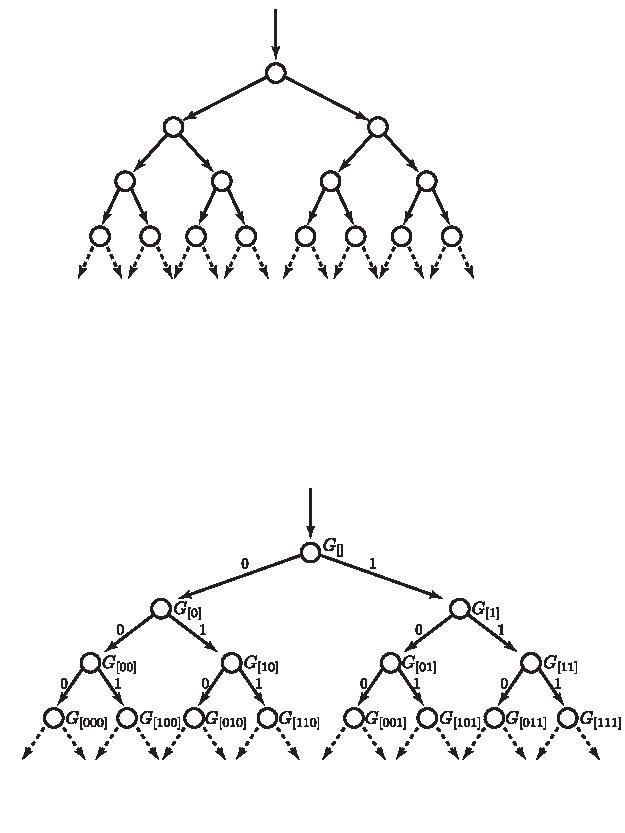
\includegraphics[width = 9cm, trim = 1cm 1cm 1cm 10cm]{../figs/base.pdf}
		\end{center}
	\end{figure}
\end{frame}


\begin{frame}[t]{Generative Process: Pitman-Yor Process}

	\begin{block}{Model}
		\vspace{-.5cm}
		\begin{eqnarray*}
			\G | d,c, \G_0 &\sim& \PY(d,c,\G_0) \\
			x_i | \G &\sim& \G, \;\; i=1,\ldots,n
		\end{eqnarray*}
	\end{block}

	\begin{block}{Generative Process ($\{ x_i \}_{i = 1}^n$)}
		\begin{itemize}
			\item Draw a partition of the first $n$ natural numbers from the two parameter Ewen's Sampling Distribution ($\ES_n(d,c)$) \cite{Ewens1995}.
				\begin{itemize}
					\item {\scriptsize For example: $(1,5,6,7)(2,8)(3)(4)$}
				\end{itemize}
			\item Assign a value $\psi_t \sim \G_0$ to part $t$ of the partition.
				\begin{itemize}
					\item {\scriptsize For example: $\psi_1 = \textrm{a}, \psi_2 = \textrm{c}, \psi_3 = \textrm{t}, \psi_4 = \textrm{u}$}
				\end{itemize}			
			\item Set $x_i = \psi_t$ if $i$ is in the $t^{\rm th}$ part of the partition.
				\begin{itemize}
					\item {\scriptsize For example: $ \{ x_i \}_{i = 1}^8 = \{ \textrm{a,c,t,u,a,a,a,c} \}$}
				\end{itemize}
		\end{itemize}
	\end{block}	
\end{frame}

\begin{frame}[t]{Ewen's Sampling Distribution ($\ES_n(d,c)$)}

	\begin{block}{Drawing from $\ES_n(d,c)$}
		\begin{itemize}
			\item Assign the integer $1$ to part $1$ of the partition.
			\item {For $i = 2, \ldots, n$, assign integer $i$ to a part drawn from the following distribution: \\
				\vspace{-.65cm}
				\begin{eqnarray*}
					p({\rm part~}t \leq k_{i-1}  | {\rm previous~assignments}) &=& \frac{n^{i-1}_t - d}{i-1 + c}\\
					p({\rm  part~} k^{i-1} + 1 | {\rm previous~ assignments}) &=& \frac{k^{i-1}d + c}{i-1 + c}\\
				\end{eqnarray*}
				\noindent where $k^{i-1}$ is the number of partitions to which the first $i-1$ integers have been assigned and $n^{i-1}_t$ is the number of integers $< i$ assigned to part $t$.
			}
			\item{Resulting partition follows $\ES_n(d,c)$  \cite{Pitman1995}}.
		\end{itemize}
	\end{block}
	
\end{frame}

\begin{frame}[t]{Chinese Restaurant Process}
	
	\begin{block}{CRP Analogy}
			Consider $n$ customers entering a giant Chinese restaurant sequentially
			\vspace{.25cm}
		\begin{itemize}
			\item Customer $i$ enters the restaurant
			\item The probability she joins an occupied table is $\frac{i-1 - (k^{i-1}d)}{i-1+c}$
			\item If she chooses to join an occupied table, she chooses table $t$ with probability proportional to $n_t^{i-1} - d$
			\item Otherwise she sits by herself
		\end{itemize}
			\vspace{.25cm}		
		The final seating arrangement corresponds to a partition drawn from the $\ES_n(d,c)$ distribution.
	\end{block}
	
\end{frame}

\begin{frame}[t]{Hierarchical Pitman-Yor Process Language Model (HPYPLM)\cite{teh2006a}}

	\begin{block}{Model}
		\vspace{-.5cm}
		\begin{eqnarray*}
			\G_{\vec {\bf u}} | d_{| \vec \bu |}, c_{| \vec \bu |}, \G_{\sigma(\vec \bu)} &\sim& \PY(d_{| \vec \bu |}, c_{|\vec  \bu |}, \G_{\sigma(\vec \bu)}) \\
			x_i | \G_{[x_{max({i-k-1,0})}, x_{i-k+1}, \ldots, x_{i-1}]} &\sim& \G_{[x_{max({i-k-1,0})}, x_{i-k+1}, \ldots, x_{i-1}]}\\
			\sigma([x_1, x_2, \ldots, x_m]) &=& [x_2, x_3, \ldots, x_m]\\
			\G_{\sigma([])} &=& \mathcal{U}_\Sigma
		\end{eqnarray*}
	\end{block}
	
		\begin{block}{Generative Process ($\{x_i\}_{i = 1}^n \sim \G_\bu$)}
		\begin{itemize}
			\item Draw a partition of the first $n$ natural numbers from the two parameter Ewen's Sampling Distribution ($\ES_n(d,c)$) \cite{Ewens1995}.
			\item Assign a value $\psi_t \sim \G_{\sigma(\bu)}$ to part $t$ of the partition.
			\item Set $x_i = \psi_t$ if $i$ is in the $t^{\rm th}$ part of the partition.
		\end{itemize}
	\end{block}
\end{frame}

\begin{frame}[t]{Hierarchical CRP}

	\begin{block}{Hierarchical CRP}
		The Chinese restaurant analogy can be hierarchically composed.  In this case it is known as the Chinese restaurant franchise.  Below is a graphical depiction of a draw from the hierarchical CRP.
	\end{block}	
		\begin{figure}[t]
		\begin{center}
			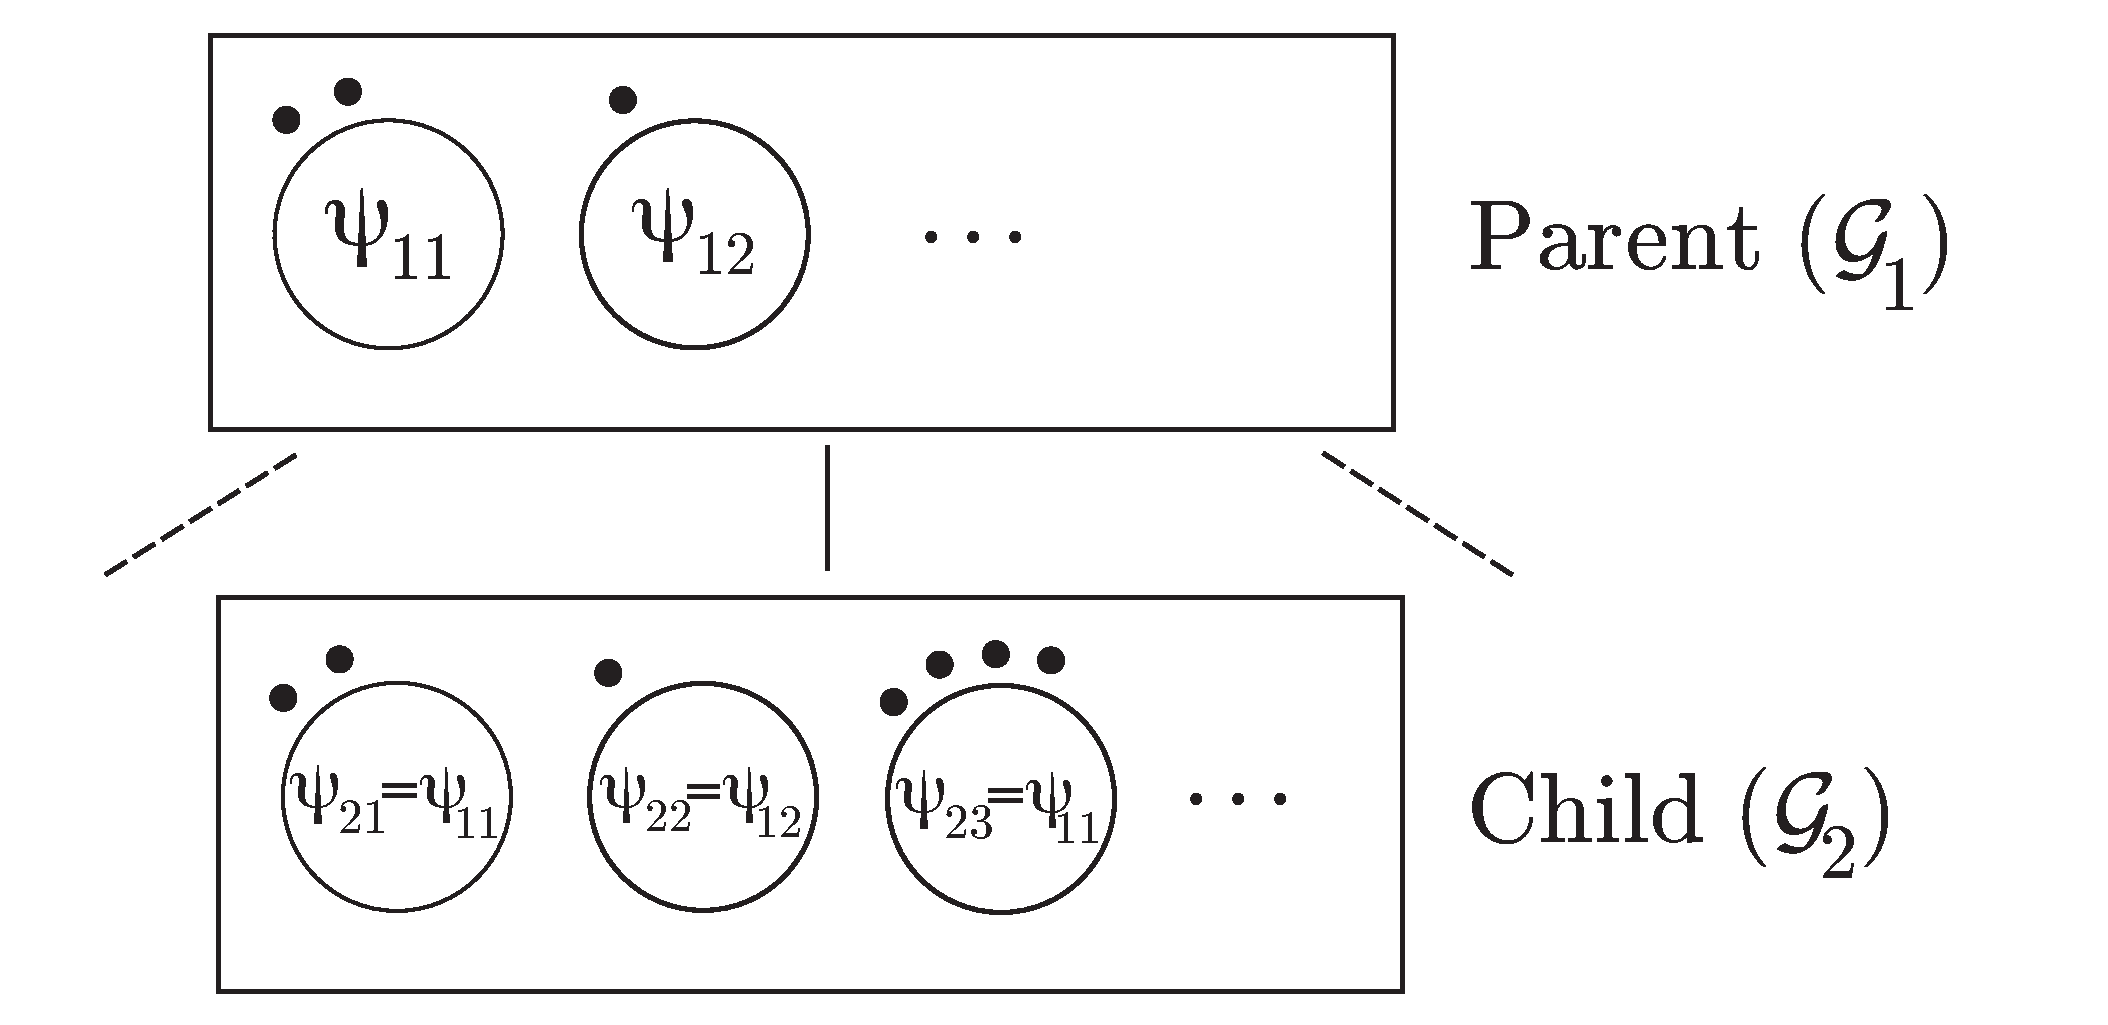
\includegraphics[width = 9cm]{../figs/figure1.pdf}
		\end{center}
	\end{figure}
\end{frame}

\begin{frame}[t]{Parameters}
	\begin{block}{Parameters ($ \{ \G_{\vec \bu} \}_{\vec \bu \in \Sigma^k}$)}
		\begin{itemize}
			\item The generative procedure is described by the Chinese franchise process
			\item Inference can be restricted to the mechanics of the generative procedure
			\item Nodes not accessed during the generation of the training data are therefore not considered during inference
		\end{itemize}
	\end{block}	
\end{frame}

%\begin{frame}[t]{Inference}
%	\begin{block}{Gibbs}
%		\begin{itemize}
%			\item Inference is performed in the HPYPLM by using MCMC simulation of the posterior distribution.
%			\item The sampler operates on the Chinese restaurant franchise representation of the process.  
%			\item In the CRF representation the parameters are the seating arrangements in each node of the graphical model.
%			\item Nodes with no customers do not need to be considered during inference.
%		\end{itemize}
%	\end{block}
%\end{frame}
%

\begin{frame}[t]{HPYPLM graphical model}
	
	Consider the nodes required for the string ``oacac" where $k$ is large: 
	\begin{figure}[t]
		\begin{center}
			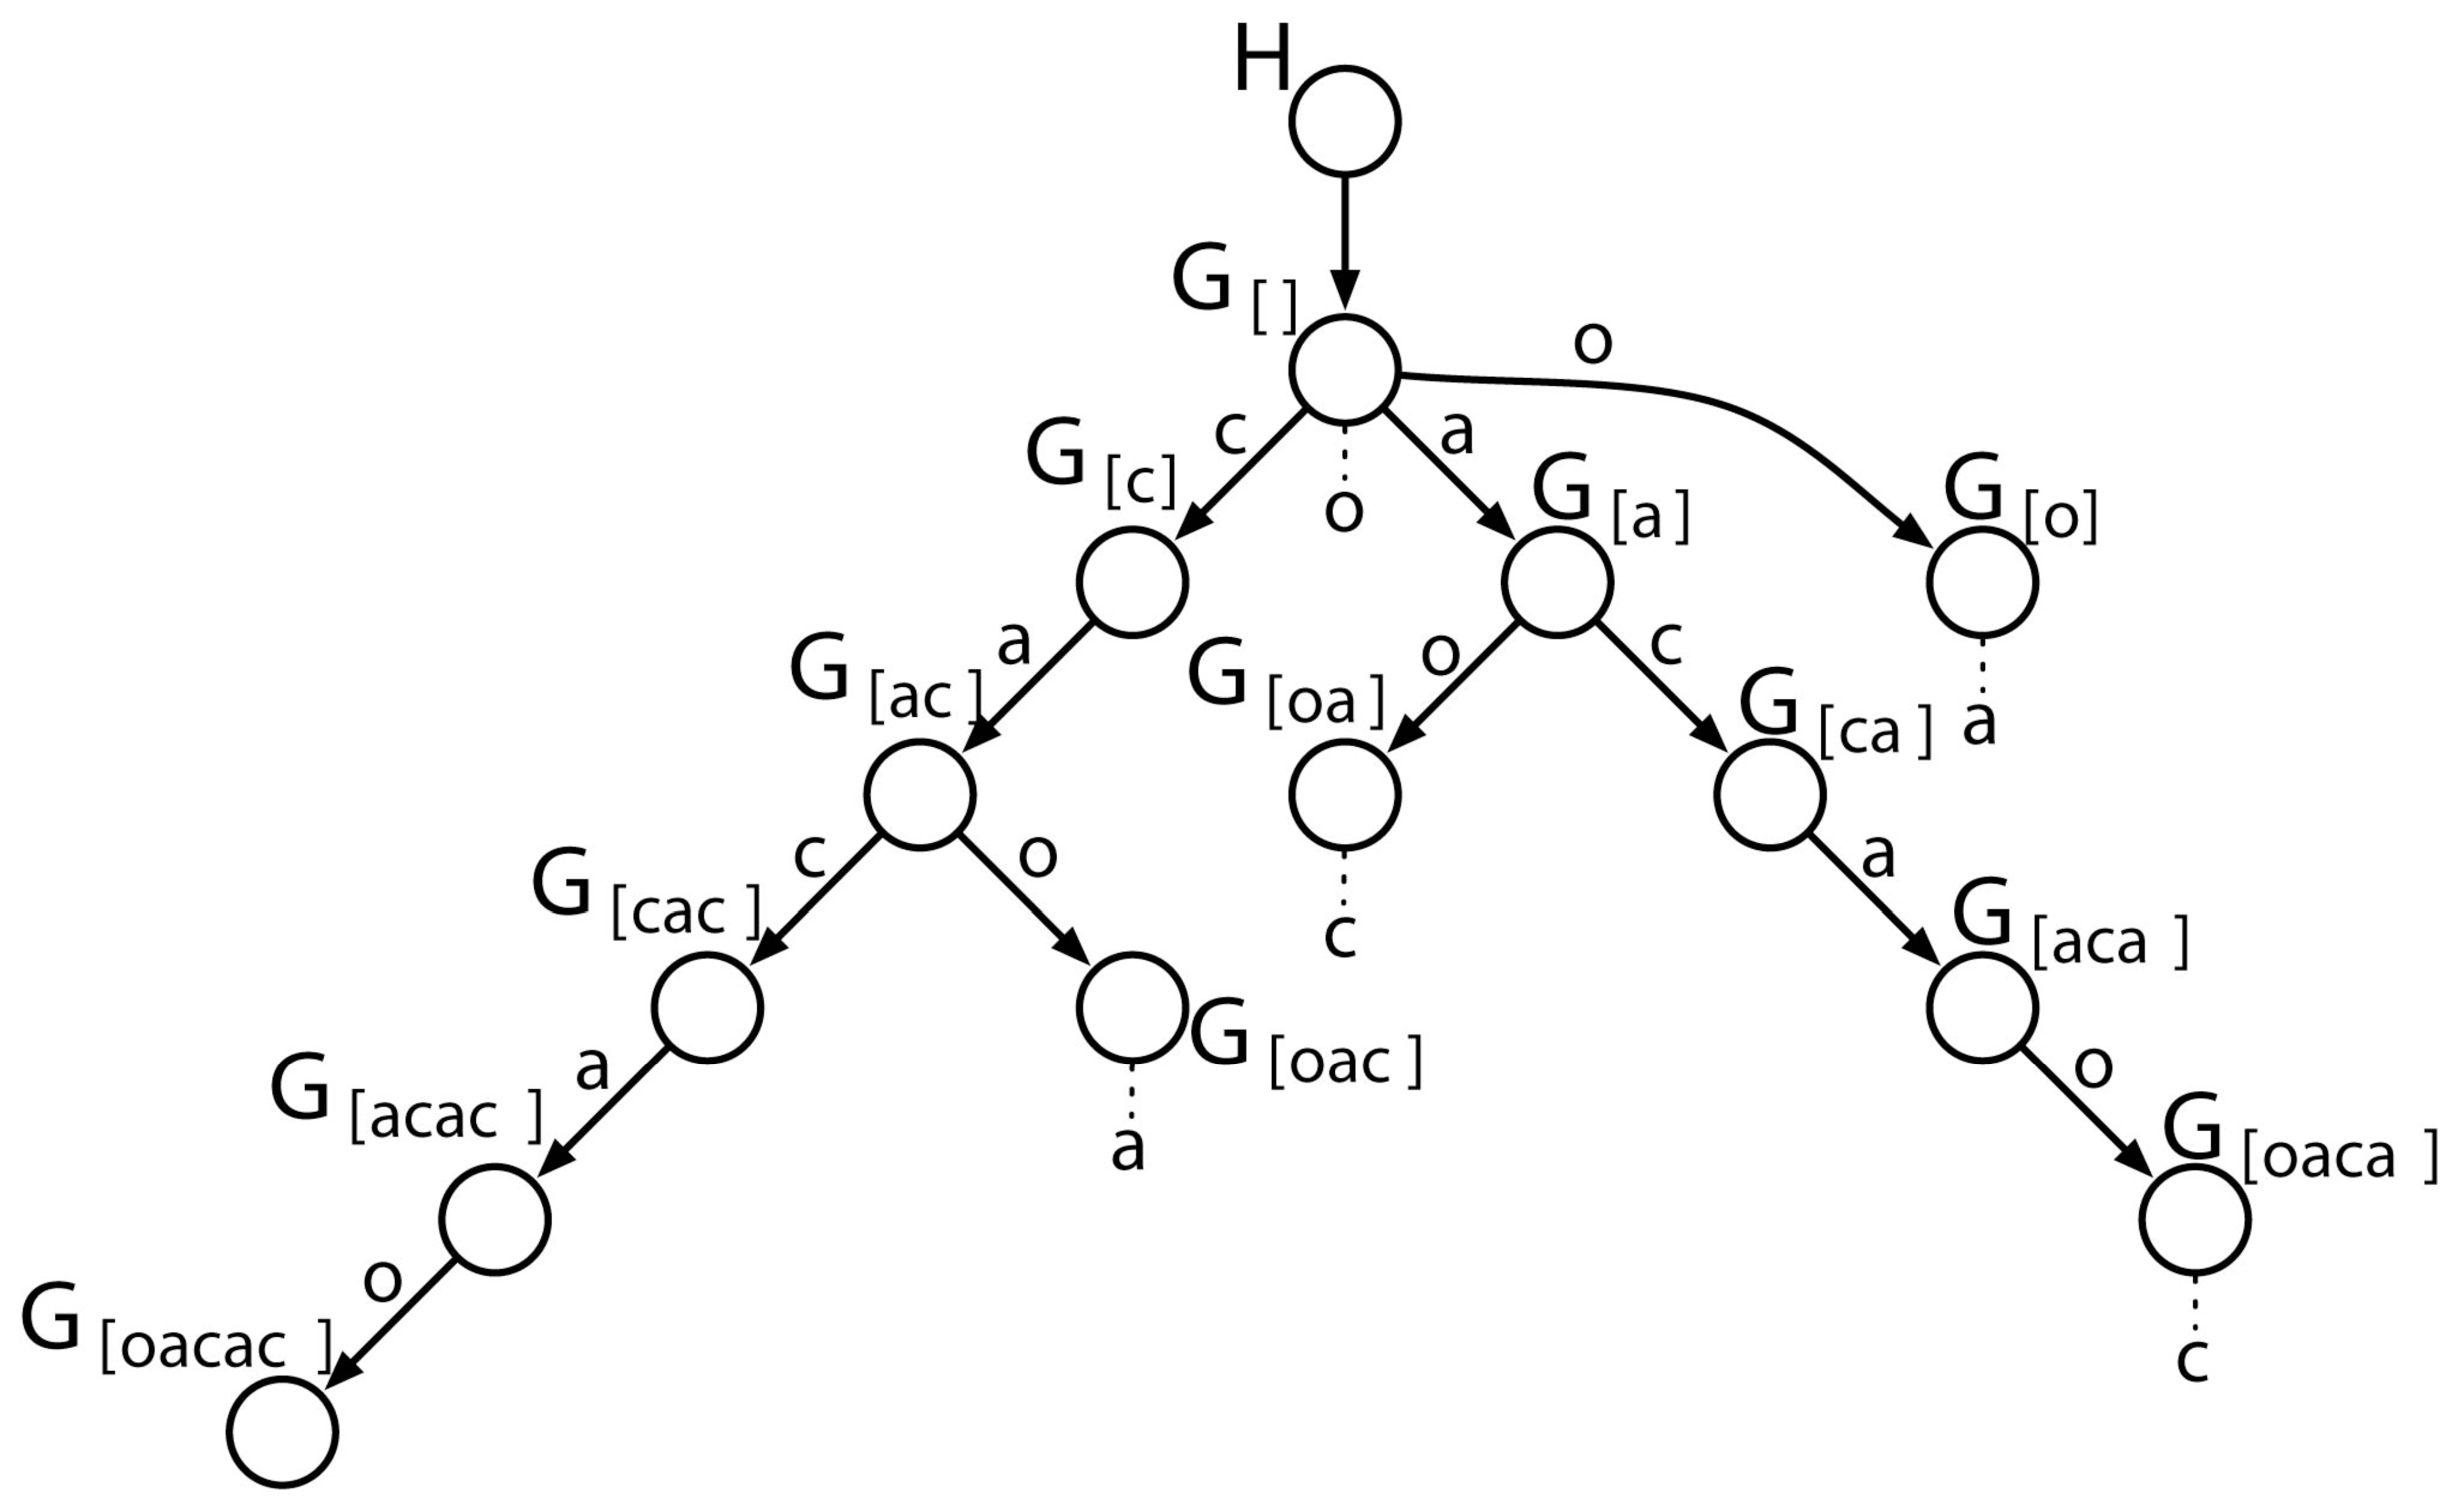
\includegraphics[height = 6cm]{../figs/prefix_trie_not_coloured.pdf}
		\end{center}
	\end{figure}
\end{frame}

%\begin{frame}[t]{HPYPLM Complexity}
%	\begin{block}{Complexity}
%		\begin{itemize}
%			\item At a fixed depth, the complexity of inference in the HPYPLM grows linearly.  
%			\item With an infinite depth, the complexity grows quadratically.
%			\item But ... as the depth of the model grows, the predictive power grows.
%		\end{itemize}
%	\end{block}
%\end{frame}


\begin{frame}[t]{Sequence Memoizer \cite{Wood2009}}
	\begin{block}{Sequence Memoizer (SM)}
		\begin{itemize}
			\item With some improvements, the infinite depth HPYPLM is known as the Sequence Memoizer model \cite{Wood2009}
			\item Spacial complexity is linear in the length of the sequence
			\item Incremental estimation and construction is quadratic in length of the sequence (though linear in real world data) \cite{Gasthaus2010}
		\end{itemize}
	\end{block}

        \begin{block}{Improve on Linearity}
          \begin{itemize}
            \item Linear space is better, but intractable for streaming data
            \item Introduce forgetting / dependent model
            \item Approximate model predictive power
          \end{itemize}
        \end{block}
\end{frame}

\section{Dependent HPYP}
%\subsection{}

\begin{frame}[t]{Consistency of $\ES$ Under Deletion}
	\begin{block}{Property}
		If an integer is removed at random from a partition following $\ES_n(d,c)$ the resulting partition of $n-1$ integers follows $\ES_{n-1}(d,c)$  \cite{Pitman1995}.
	\end{block}
	
	\begin{block}{Application}
		This consistency property can be exploited in a generative procedure defined using the Chinese restaurant representation to draw samples from a sequence of dependent distributions $\{ \G^t \}_{t = 1}^T$ such that 
		\[
		\begin{array}{rcll}
			\G^t | d,c,\G_0 &\sim& \PY(d,c,\G_0)& t = 1, \ldots, T\\
			X_i^t | \G^t &\sim& \G^t& i = 1, \ldots, n^t, t = 1, \ldots, T
		\end{array}
		\]
	\end{block}
\end{frame}

\begin{frame}[t]{Dependent PYP}
	\begin{block}{Model}
		\vspace{-.5cm}
		\begin{eqnarray*}
			G^t | d,c, G_0 &\sim& \PY(d,c,G_0) \\
			x^t_i | G^t &\sim& G, \;\; i=1,\ldots,n^t
		\end{eqnarray*}
	\end{block}

	\begin{block}{Generative Process}
		\begin{itemize}
			\item For $t = 1$, draw a size  $n^1$ sample as in PYP.
			\item Between time steps, remove objects from the partition.
			\item To generate a sample at time $t$, add $n^t$ objects to the partition following the sequential generative process of the $\ES(d,c)$.
			\item Assign a random draw from $G_0$ to any new parts.  Sample elements are given values according to the location of the $n^t$ newly placed objects.
			\item This process is an extension of GPU DDP \cite{Caron2007}.
		\end{itemize}
	\end{block}
\end{frame}

\begin{frame}[t]{Dependent HPYP (\citet{Bartlett2010})}
	
	\begin{block}{HPYP}
		\begin{itemize}
			\item The dependent generative process can be extended to the HPYP.
			\item Deletion may only occur in leaf restaurants.
			\item A leaf restaurant is one such that all restaurants in the subtree stemming downward are empty.
		\end{itemize}

	\end{block}
\end{frame}

\begin{frame}[t] {Depiction of Dependent HPYP}
	\begin{figure}[t]
		\begin{center}
			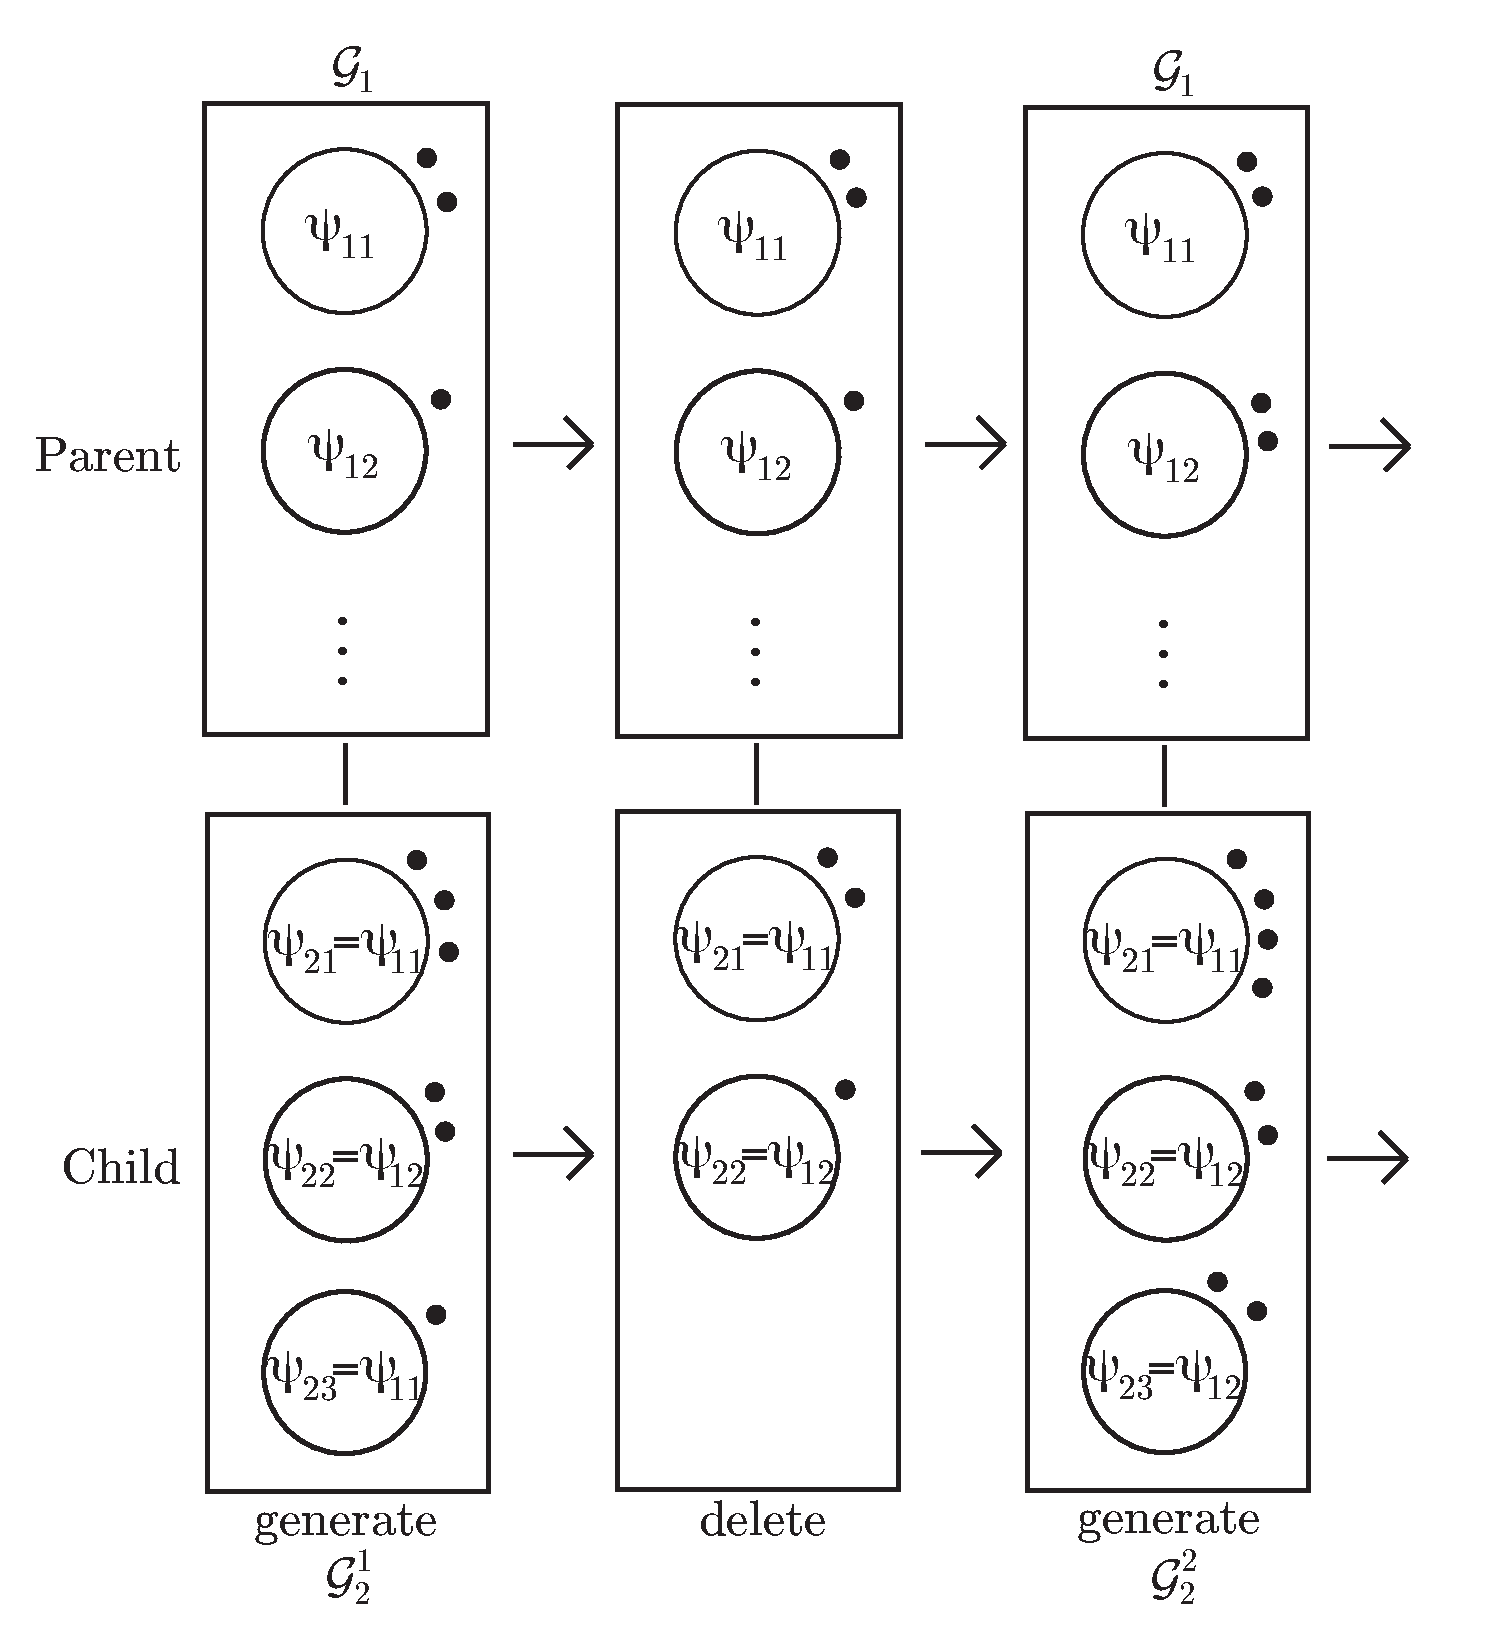
\includegraphics[height = 7cm]{../figs/figure2.pdf}
		\end{center}
	\end{figure}
\end{frame}

\begin{frame}[t]{Deletion}
	\begin{block}{Notes about deletion}
		\begin{itemize}
			\item The number of customers deleted during the deletion step is independent of the consistency result.
			\item The number of customers deleted from a given restaurant can be either deterministic or stochastic.
			\item Only customers in leaf restaurants may be deleted during the deletion step.
		\end{itemize}
	\end{block}
	
	\begin{block}{Constant Space (\citet{Bartlett2010})}
		\begin{itemize}
			\item A generative procedure which deterministically deletes all customers in a chosen leaf restaurant is well specified.  Since empty restaurants are not represented during inference, such a model can be used to limit the number of instantiated restaurants and allow for constant space representation.
			\end{itemize}
	\end{block}
\end{frame}

%\subsection{}

%\begin{frame}[t]{Description}
%	\begin{block}{Compression}
%		\begin{itemize}
%			\item The Sequence Memoizer, an infinite order HPYP,  is an effective predictive model for the task of compression \cite{Gasthaus2010}.
%			\item Files are modeled as a sequence of bytes.
%			\item The linear space requirement of the SM prohibits it's use on large files.
%		\end{itemize}
%	\end{block}
%	
%	\begin{block}{DHPYP for Compression}
%		\begin{itemize}
%			\item We create a dependent SM for the task of compression.
%			\item We control the amount of space required by the model by the number of instantiated restaurants.
%			\item Inference is performed using  a single particle particle filter, a technique which works well with the SM \cite{Gasthaus2010}.
%		\end{itemize}
%	\end{block}
%\end{frame}
%
%\begin{frame}[t]{Constant Space Sequence Memoizer}
%	\begin{figure}[t]
%		\begin{center}
%			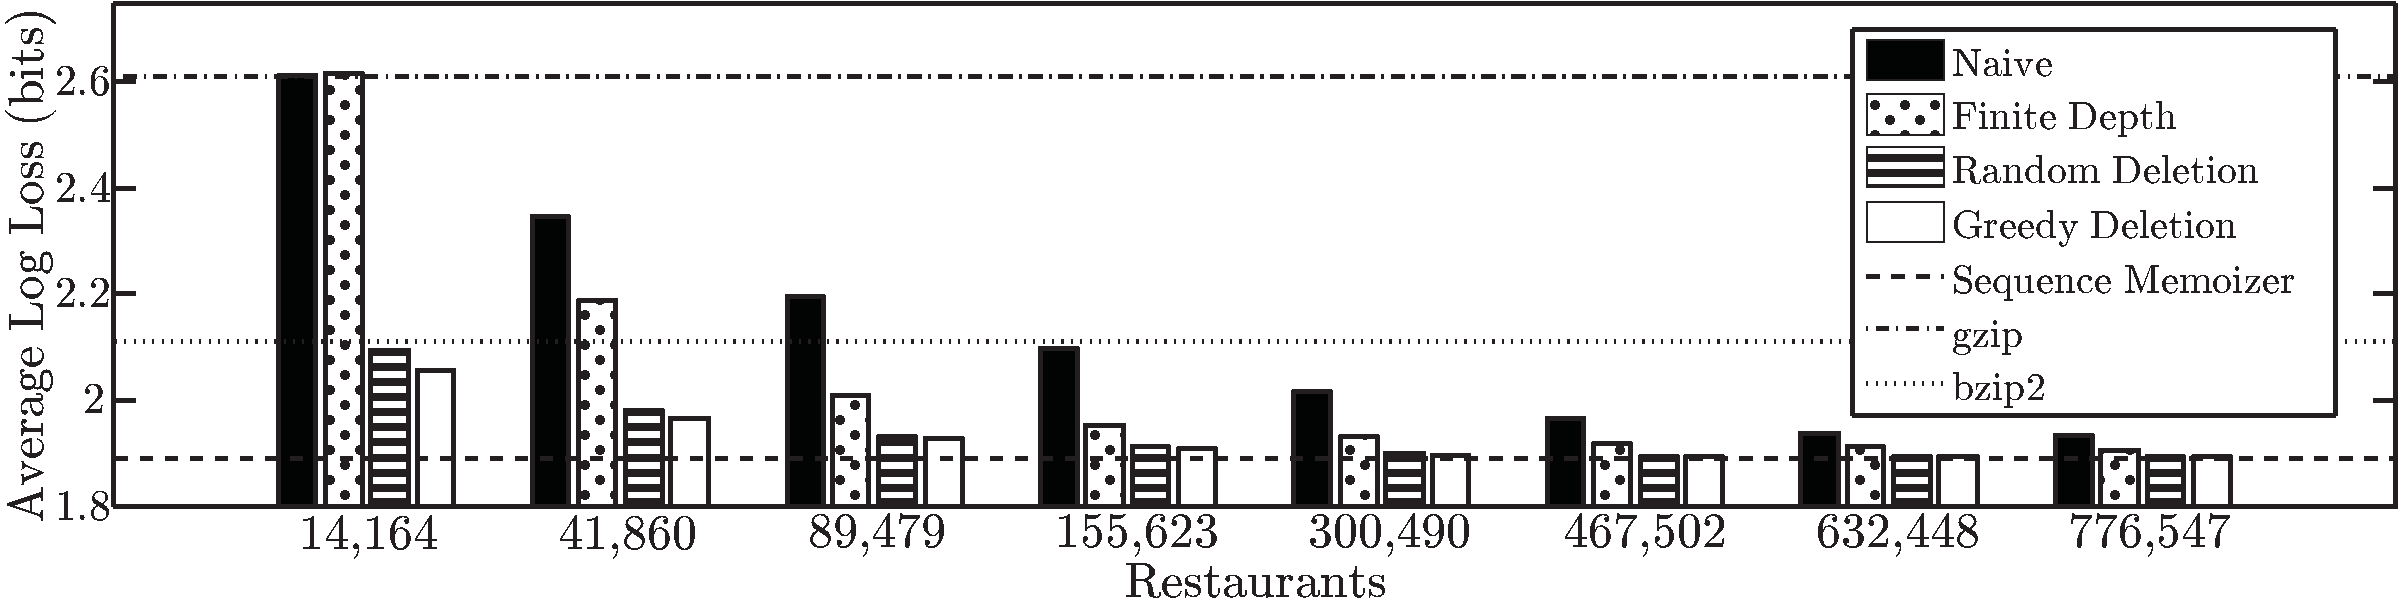
\includegraphics[width=10cm]{../figs/results_calgary_corpus.pdf}
%		\end{center}
%	\end{figure}
%	
%	\begin{itemize}
%		\item Horizontal axis is memory, measured in restaurants.
%		\item Vertical axis is the average negative log loss of the data.
%		\item Calgary corpus (14 files, max size = 769kb).
%		\item Two forgetting schemes and two other constant space modeling approaches.
%		\item $256$ character alphabet.
%		\item SM requires 1.16 million instantiated restaurants.
%	\end{itemize}
%\end{frame}

\section{Approximations}
%\subsection{}

\begin{frame}[t]{Compressed Representation}
	
	\begin{block}{Compressed Representation \cite{Gasthaus2011}}
		\begin{itemize}
			\item The full ``seating arrangement" need not be maintained in every node.
			\item At each node, customer and table counts for each type are sufficient for most operations.
			\item The full seating arrangement is required for fragmentation.
			\item A full seating arrangement can be sampled using a forward backward algorithm.
		\end{itemize}
	\end{block}
	
\end{frame}

\begin{frame}[t]{Compressed Representation Approximation  (\citet{Bartlett2011})}
	
	\begin{block}{Compressed Representation Approximation}
		\begin{itemize}
			\item Simulation of the full seating arrangement requires computation proportional to the customer count of that type in the node.
			\item The count of customers in each node grows unboundedly.
			\item Solution : approximate the process by limiting the total number of customers ($K$) in each node of the graphical model.
			\item The upper bound $K$ is enforced through random deletion, the effect of which has already been characterized in our discussion of the DHPYP.
		\end{itemize}
	\end{block}
	
\end{frame}

\begin{frame}[t]{Suffix Tree Approximation (\citet{Bartlett2011})}

	\begin{block}{Suffix Tree}
		\begin{itemize}
%			\item The deletion of nodes means that inference is only required in a constant number of node
           \item Suffix tree data structures use pointers into the original sequence to label the edges
			\item Suffix tree data structures require linear space
			\item The suffix tree is approximated by labeling edges with pointers to a length $R$ (fixed) reference sequence
			\item Edges which cannot be labeled are removed from the tree
		\end{itemize}
	\end{block}
	
\end{frame}

\begin{frame}[t]{Suffix Tree Approximation  (\citet{Bartlett2011})}
	
	\begin{block}{Suffix Tree Approximation}
			\begin{itemize}
				\item The reference sequence is equal to a fixed length ($R$) suffix of the input sequence
				\item As data is incorporated into the model, edges are updated to point to later sections of the reference sequence
				\item Edges which cannot be labeled are removed from the tree
            	\item Contexts which are rare are likely to be removed this way
			\end{itemize}
	\end{block}
		
\end{frame}

\begin{frame}[t]{Sequential Edge Updates}

   	\begin{figure}[t]
		\begin{center}
			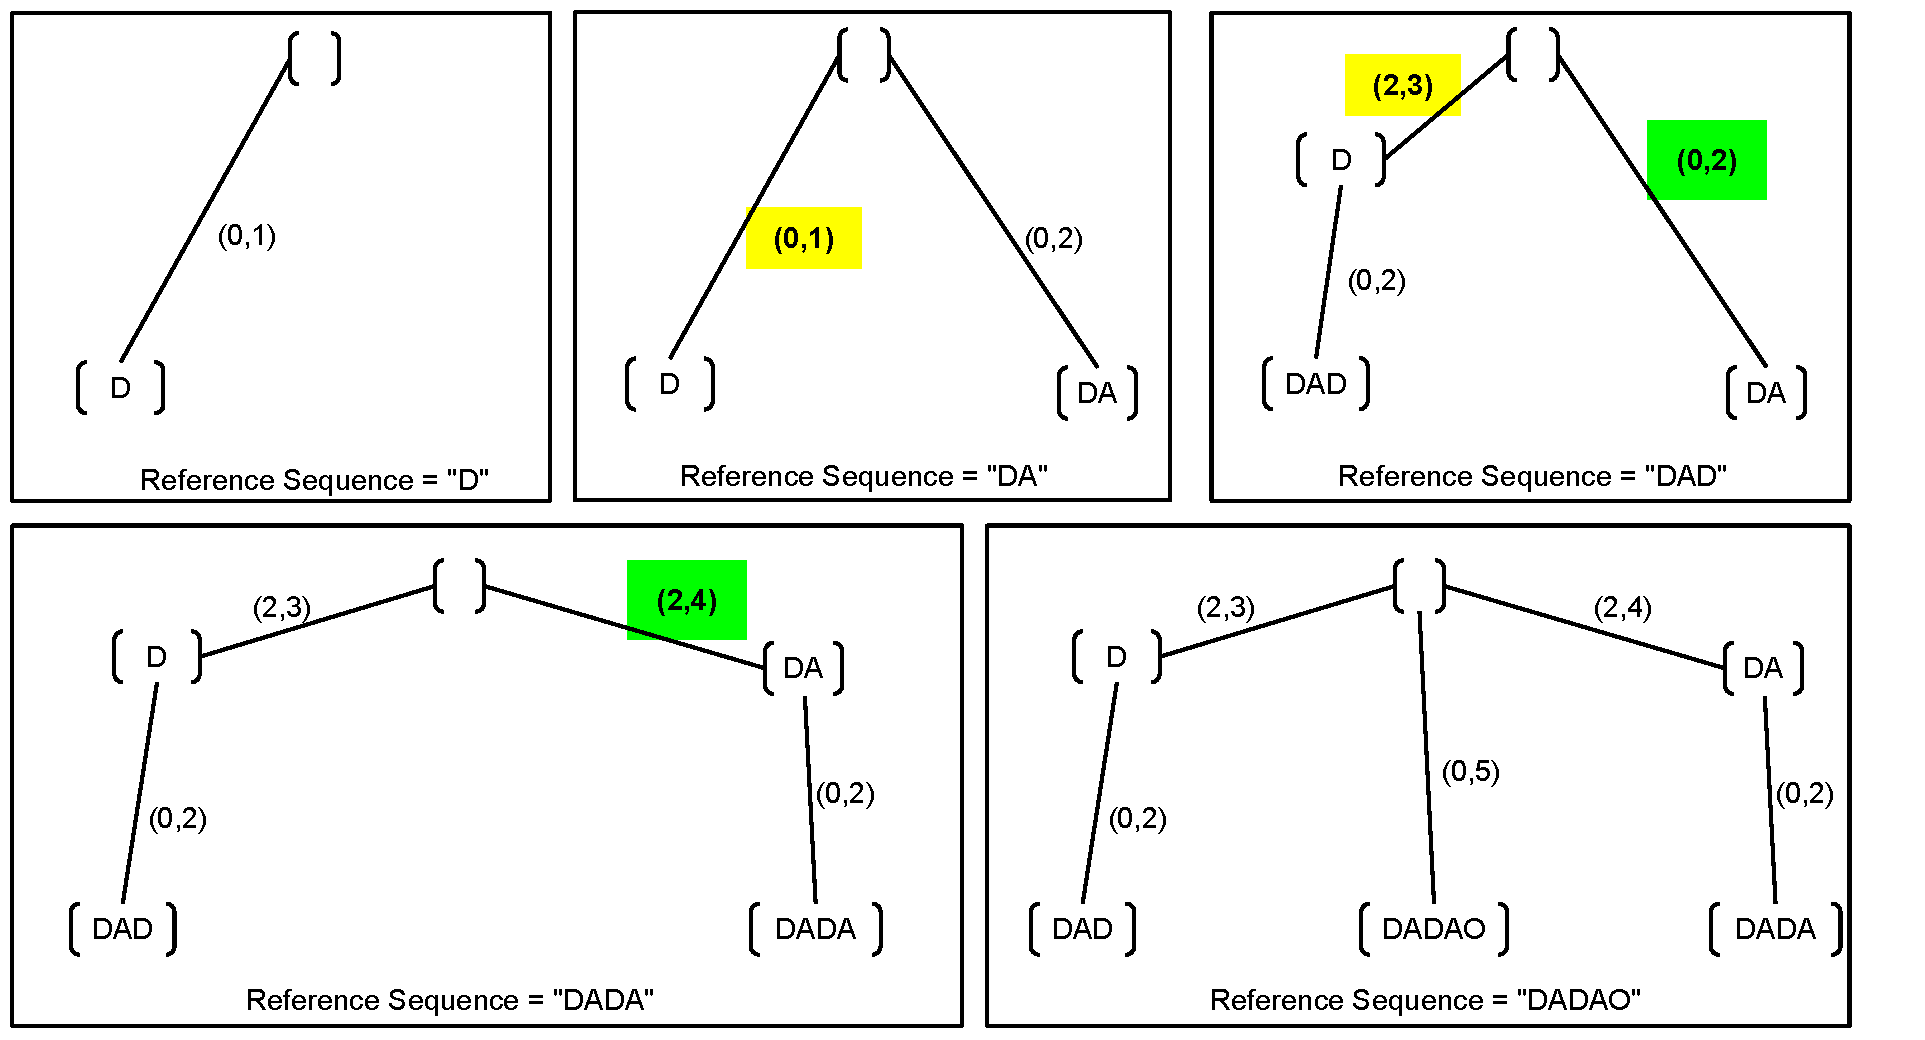
\includegraphics[width = 11cm]{../figs/DADAO.pdf}
		\end{center}
	\end{figure}

\end{frame}


\section{Experiments}
%\subsection{}

\begin{frame}[t]{Setup}
	\begin{block}{Experimental Setup}
		\begin{itemize}
			\item Data : Wikipedia .xml content dump
			\item Task : compression (incremental online prediction)
			\item Parameters of interest : stream length, node limit $L$, node size $K$, and depth of model $D$
			\item Performance Metric : compression rate (bits per byte)
		\end{itemize}
	\end{block}
\end{frame}

\begin{frame}[t]{Max count with node ($K$)}
	\begin{block}{Max count within node ($K$)}
		\begin{itemize}
			\item Tested values of $K$ in $\{2^7, 2^8, \ldots, 2^{15} \}$
			\item Performance was same for all values of $K$
			\item Experiments use $K = 2^{13} = 8,192$
		\end{itemize}
%		We varied values of $k$ between 128 and 32,768 and found that there was no discernible performance difference.  For the rest of the experiments we felt justified in fixing $k$ to 	8,192.
	\end{block}
\end{frame}


%\subsection{``Deplump for Streaming Data'' \citet{Bartlett2010}, Constant space, constant time prediction, linear time estimation SM}
\begin{frame}[t]{}
%\begin{block}{}
%\begin{figure}[htbp]
%\begin{center}
%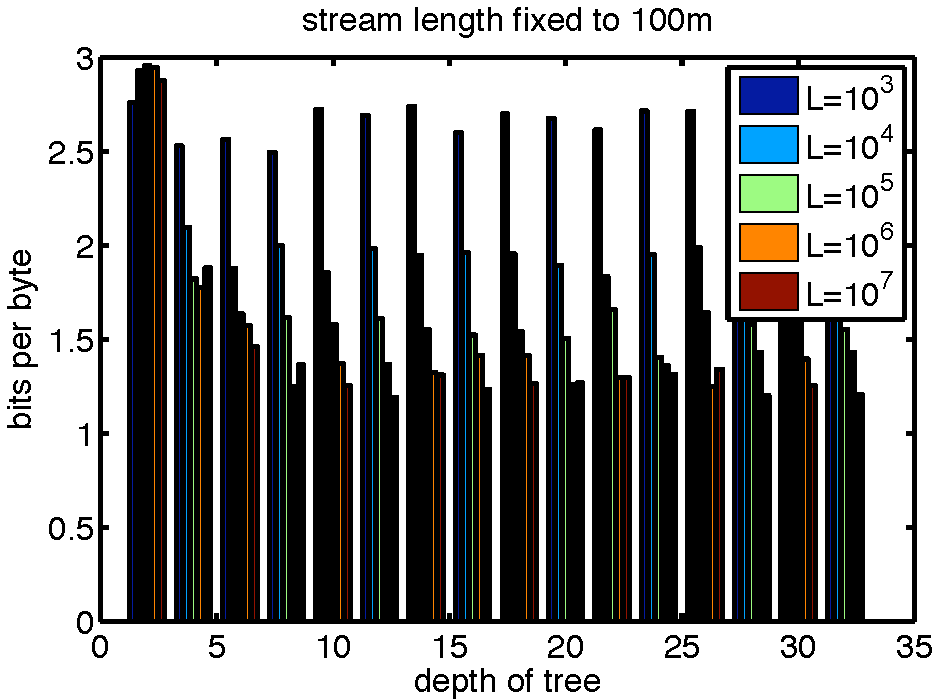
\includegraphics[width=\textwidth]{varying_depths.pdf}
%\end{center}
%\end{figure}
%A dependent HPYP can be defined though a graphical model leaf node deletion scheme.  Inference in the resulting model was shown to approximate the SM well.  \tiny{data: Calgary corpus, rests = total used nodes in 3-10 grams}
%\end{block}
\begin{figure}[htbp]
\begin{center}
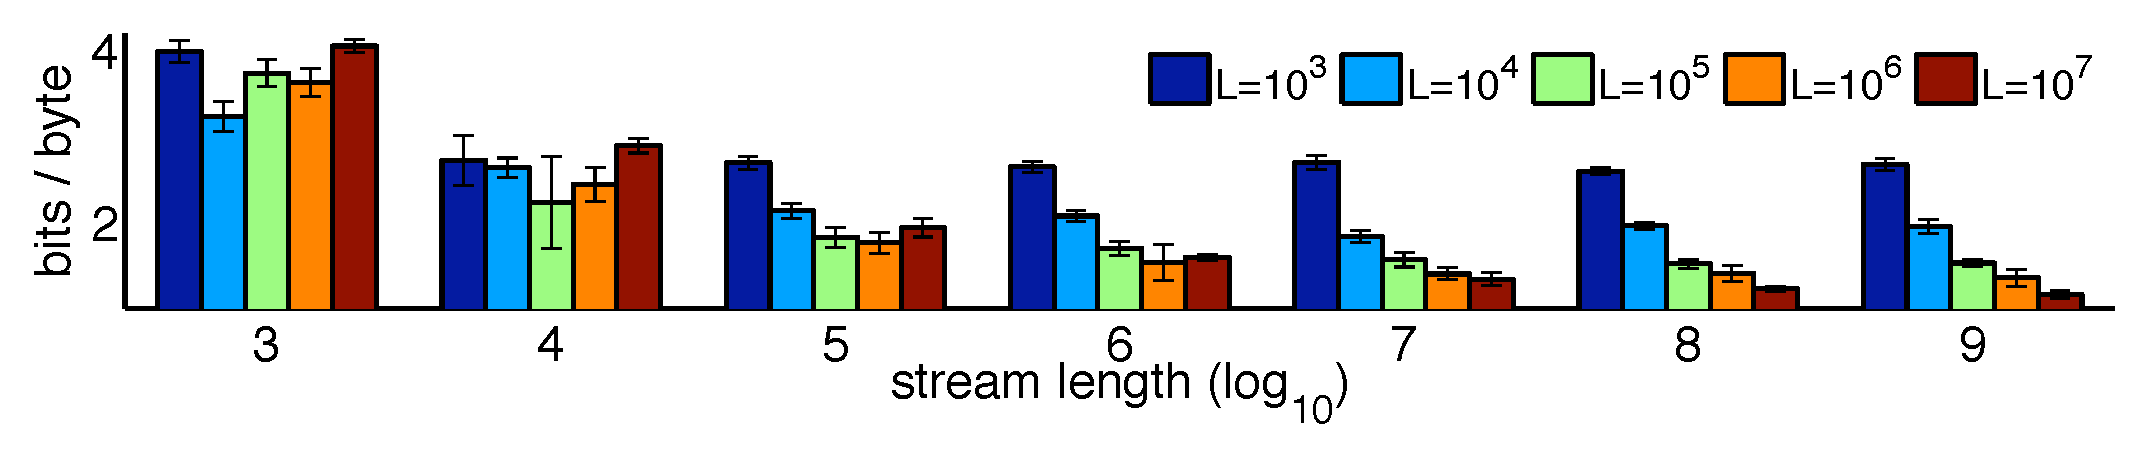
\includegraphics[width=\textwidth]{../figs/varying_stream_length.pdf}
\end{center}
\end{figure}
First streaming SM with computational asymptotics required for streaming compression.  Compressed 26.8Gb Wikipedia corpus to 4Gb (vs. 7.9Gb for gzip and 3.8Gb for PAQ).\newline
\vspace{3cm}
{\tiny $L$ is number of nodes in SM, data Wikipedia dump 2010 head, depth 16}
\end{frame}

%\begin{frame}[t]{Varying Depths}
% Average( $\pm$ std.) streaming deplump compression performance as measured in bits in compressed output vs. bytes in uncompressed input. Here the depth limit ($D$) and node limit ($L$) are varied. Results are averaged over 10 trials on sequences of length 100Mb sampled at random with replacement.
%   	\begin{figure}[t]
%		\begin{center}
%			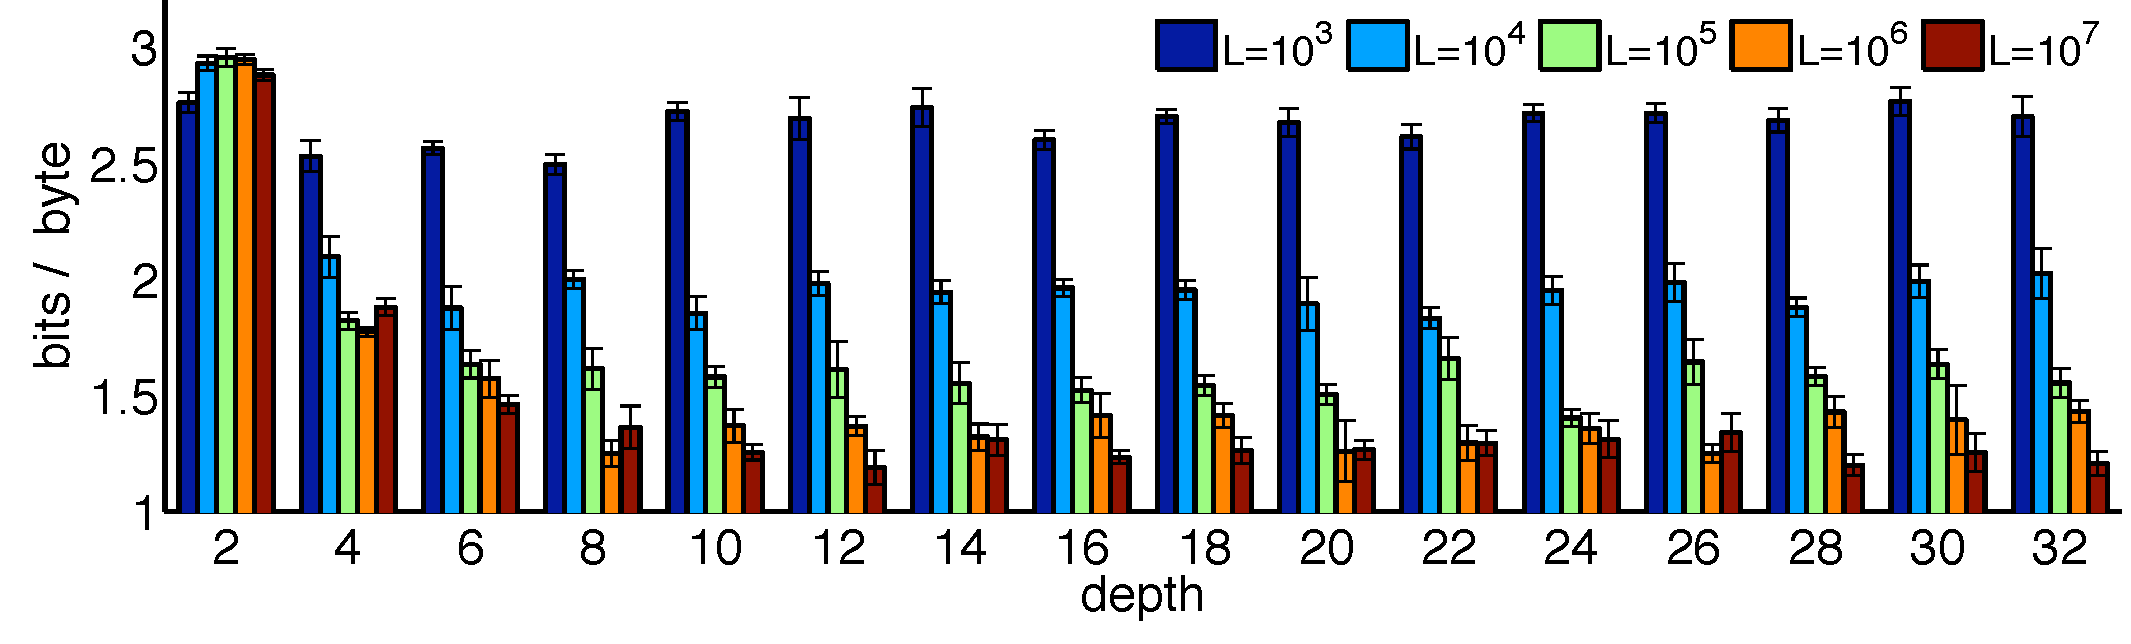
\includegraphics[width = 11cm]{../figs/varying_depths.pdf}
%		\end{center}
%	\end{figure}
%
%\end{frame}
%
%\begin{frame}[t]{Varying Stream Lengths}
%	Average ($\pm$ std.) streaming deplump compression performance as measured in bits in compressed output vs.~bytes in uncompressed input.  Here the input stream length and node limit ($L$) are varied.  From this we observe that average deplump streaming compression performance monotonically improves as the input sequence grows in length but asymptotes at a different value per node limit. Also, it can be seen that large node limits may actually hurt compression performance for small input sequences.  Depth is fixed at 16.
%	   	\begin{figure}[t]
%		\begin{center}
%			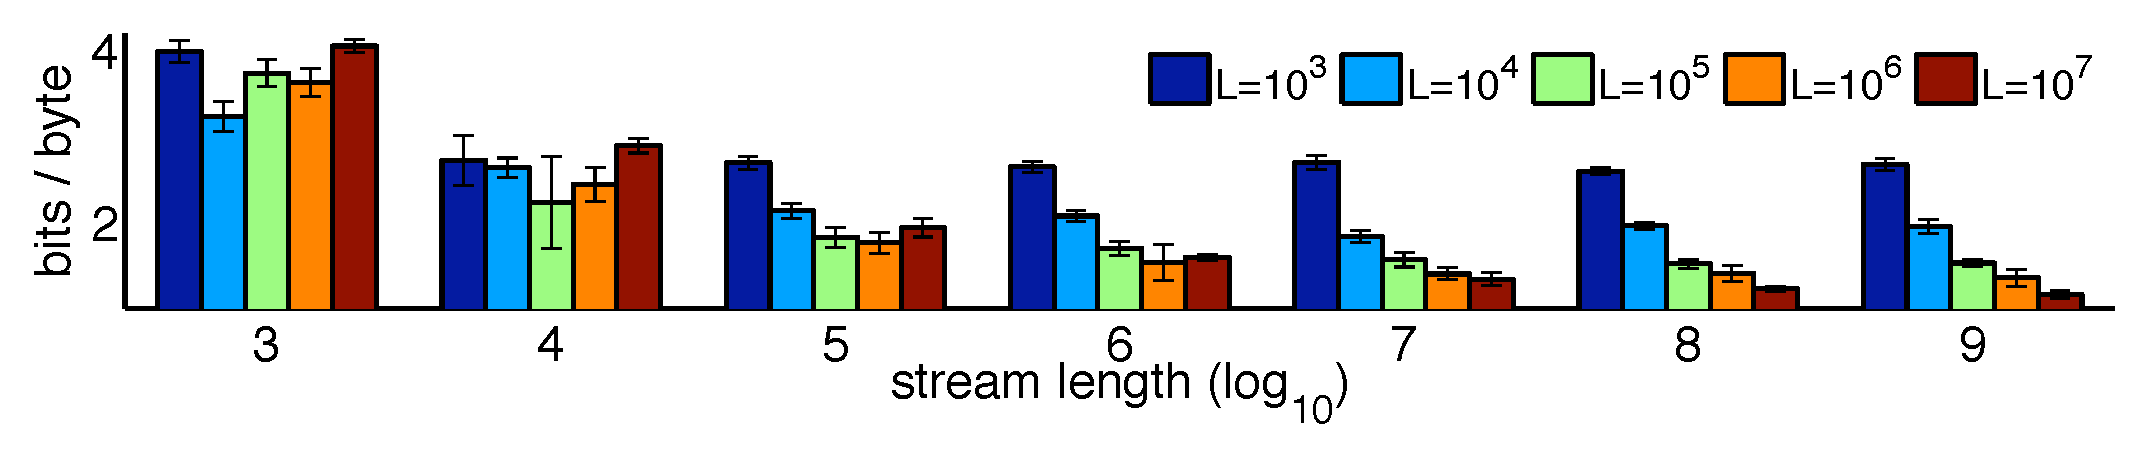
\includegraphics[width = 11cm]{../figs/varying_stream_length.pdf}
%		\end{center}
%	\end{figure}
%
%\end{frame}

%\begin{frame}[t]{Full Wikipedia Compression}
%	\begin{block}{Full Wikipedia}
%		Considering these results, we chose values for the approximating parameters of $D=32$, $L=10^7$, $k=8,192$ and compressed the full 26.8Gb Wikipedia corpus.  When compressed, the corpus was 7.8Gb gziped, 3.8Gb paq9a'ed, both with default parameters, and 4.0Gb deplumped.
%	\end{block}
%\end{frame}

\section{Discussion}
%\subsection{}

\begin{frame}[t]{Discussion}
	\begin{block}{Future Work}
		\begin{itemize}
			\item Other ways to create dependence in a sequence of HPYPs
			\item Testing of structure discovery with synthetic data
			\item Properties of single particle sequential Monte Carlo
		\end{itemize}
	\end{block}
\end{frame}

\begin{frame}[t,allowframebreaks]{Bibliograpy}
	\bibliography{../../../papers/uber}
\end{frame}

\begin{frame}[t]{HPYPLM graphical model}
	
	Consider the nodes required for the string ``oacac" where $k$ is large: 
	\begin{figure}[t]
		\begin{center}
			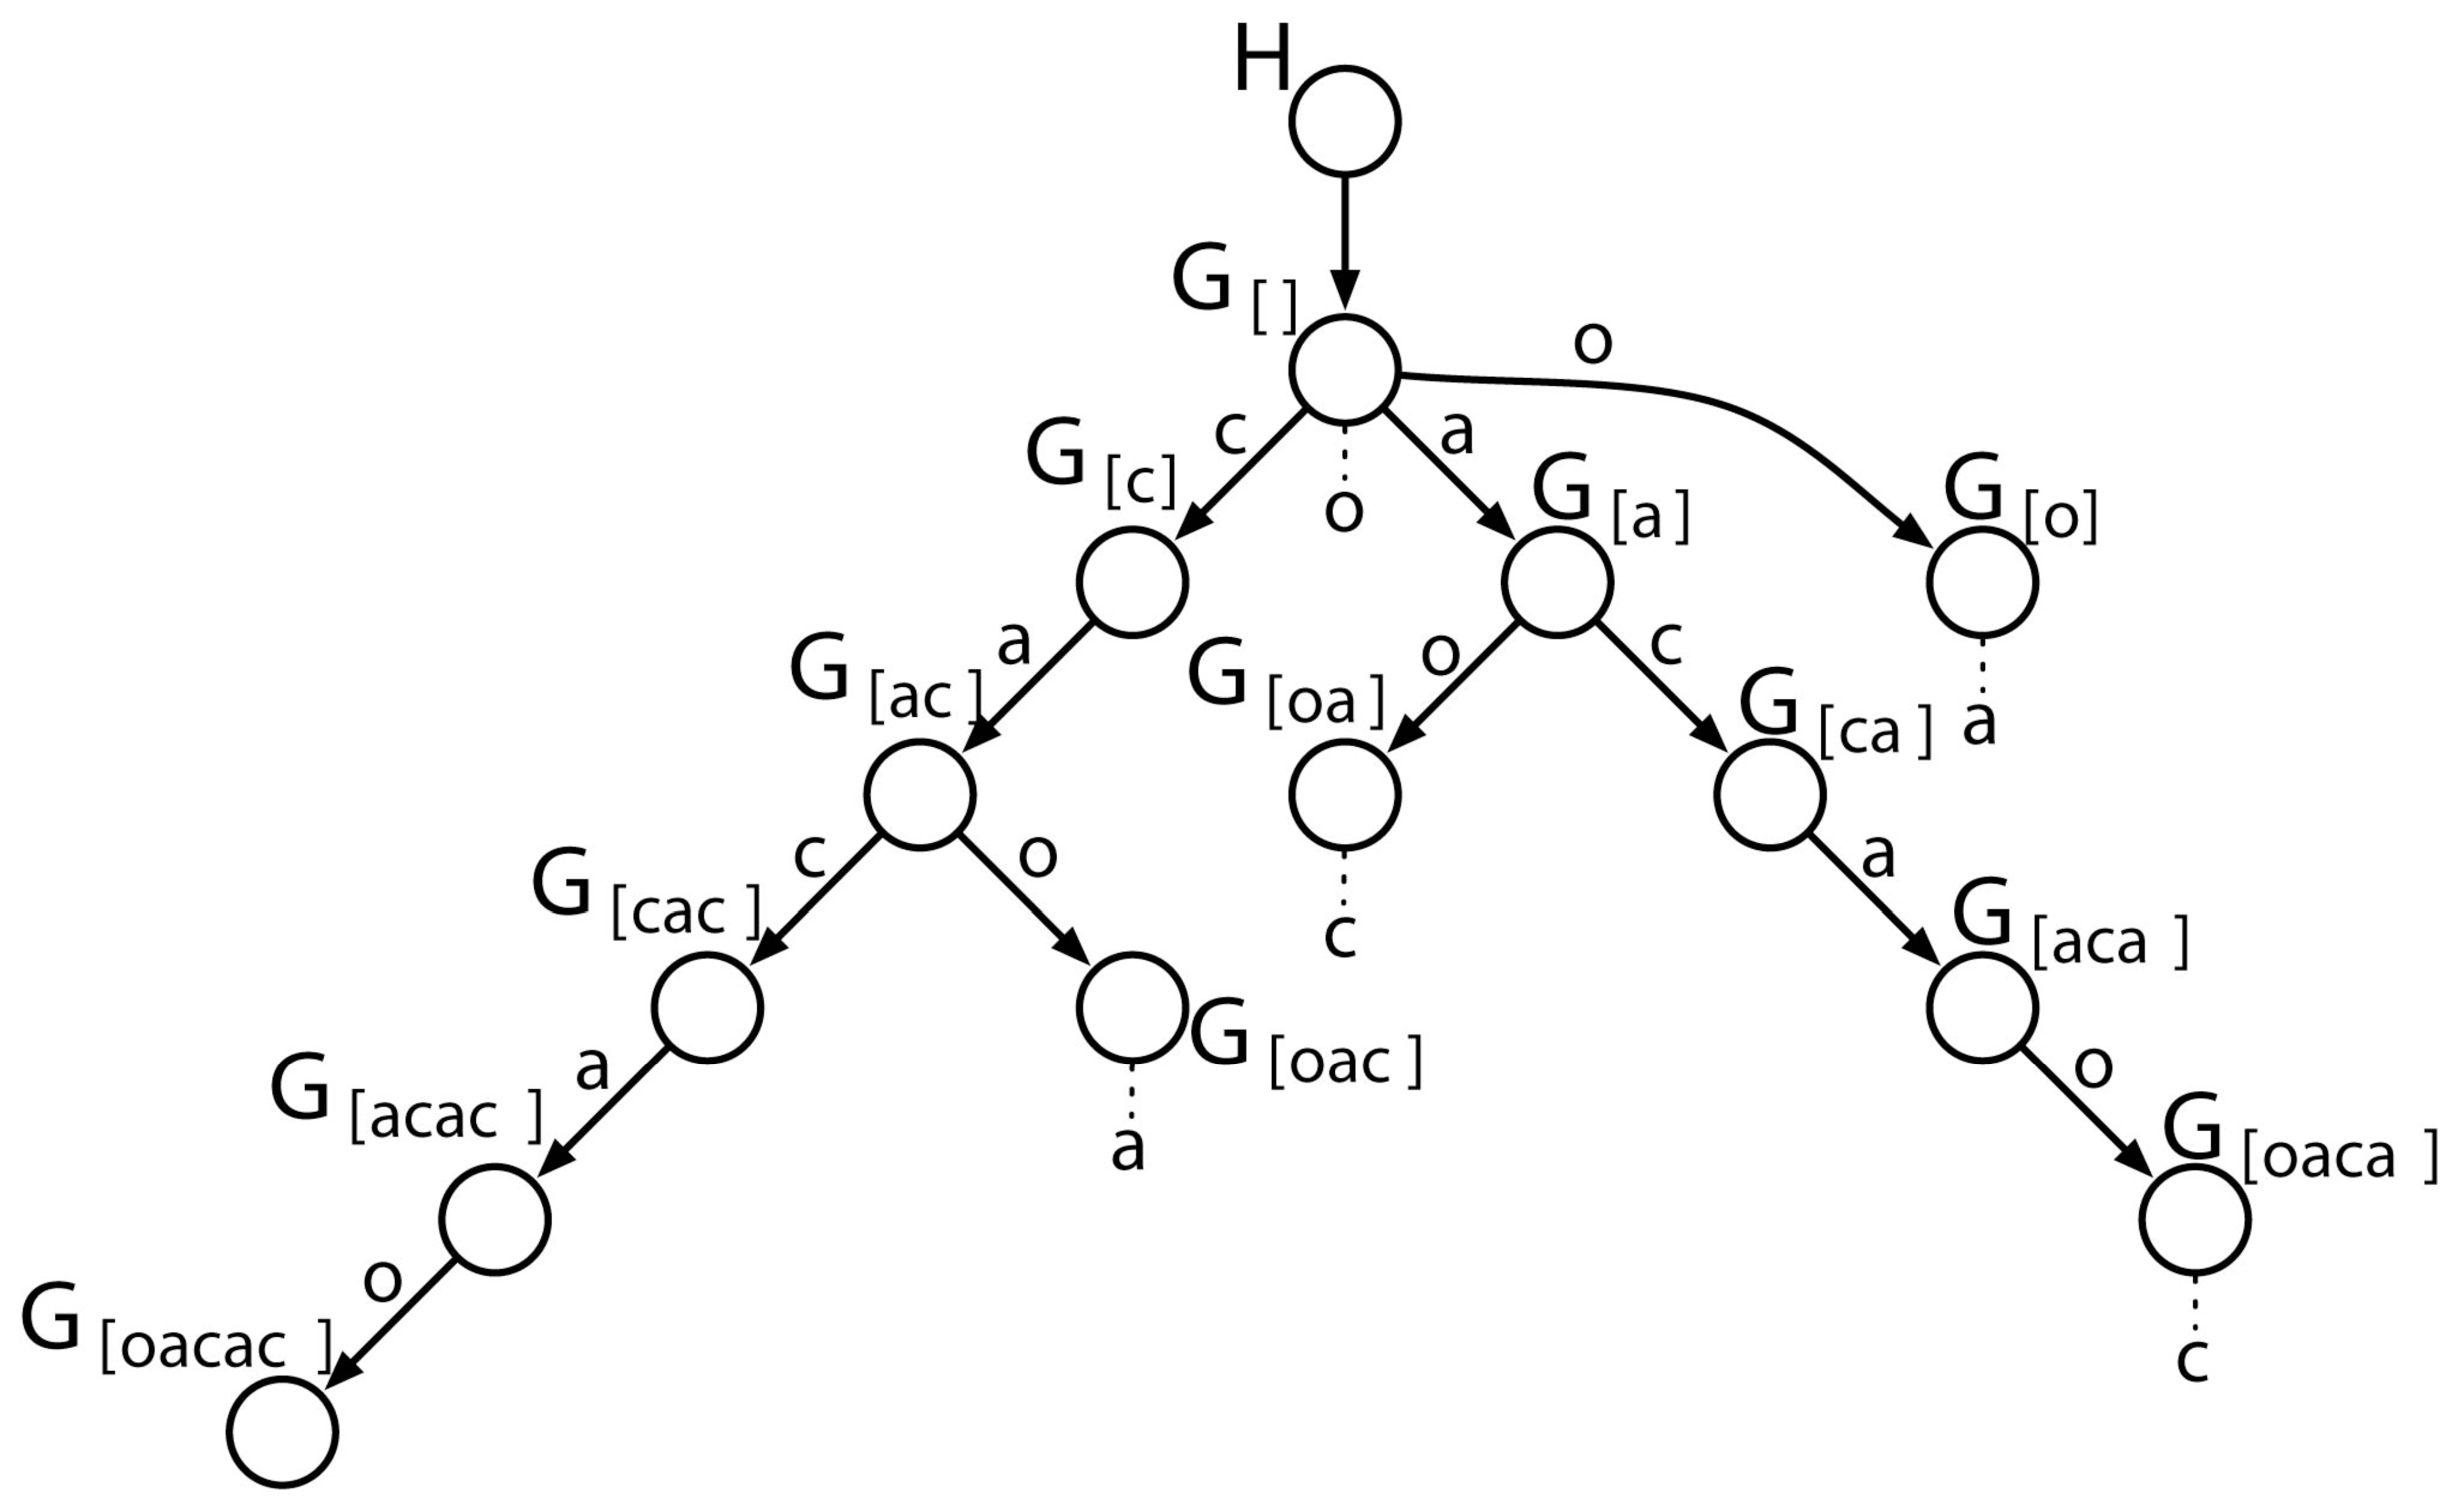
\includegraphics[height = 6cm]{../figs/prefix_trie_not_coloured.pdf}
		\end{center}
	\end{figure}
\end{frame}

\begin{frame}[t]{Marginalization}
	\begin{block}{Marginalization \cite{Pitman1999}}
		If $P(\G_1, \G_2)$ is defined by
		\begin{eqnarray*}
			P(\G_1) &=&  \PY(d_1, 0, \G_0) \\
			P(\G_2 | \G_1) &=& \PY(d_2, 0, \G_1)
		\end{eqnarray*}
		then marginally 
		\begin{eqnarray*}
			P(\G_2) =  \PY(d_1 d_2, 0, \G_0)
		\end{eqnarray*}
	\end{block}	
\end{frame}

\begin{frame}[t]{Sequence Memoizer graphical model ``oacac" ($\mathcal{O}(n)$) \cite{Wood2009}}

	\begin{figure}[t]
		\begin{center}
			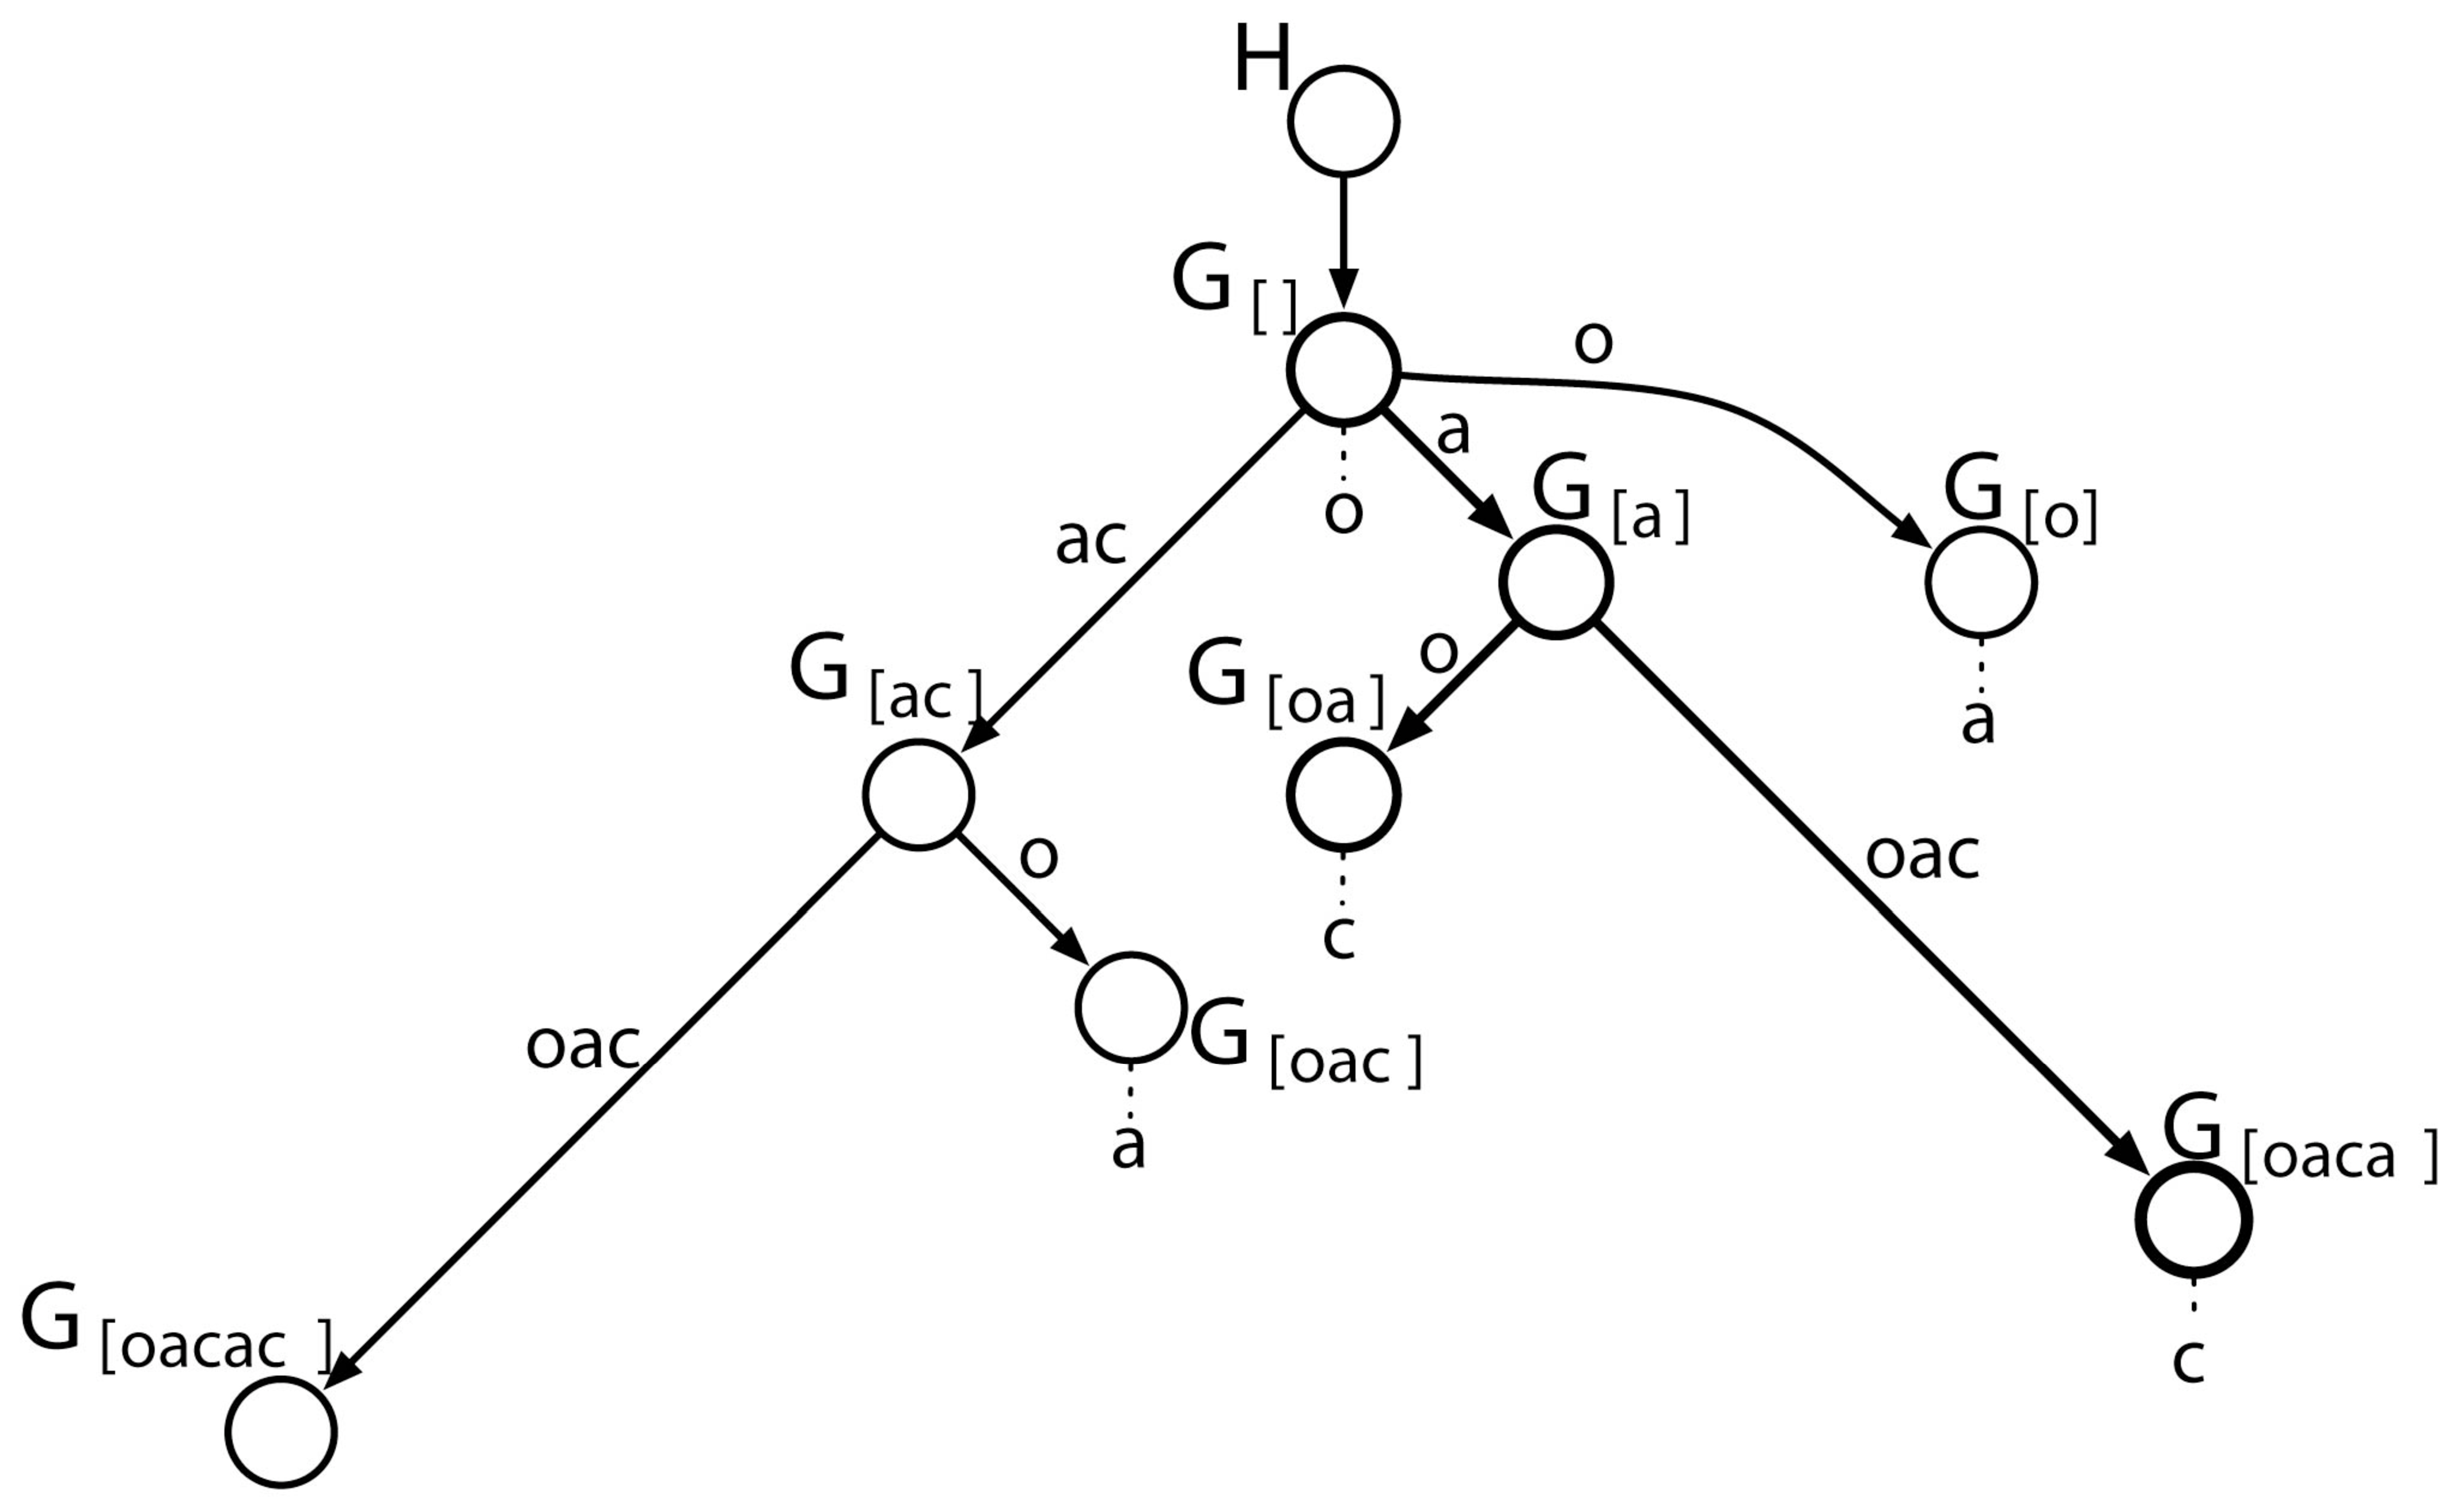
\includegraphics[height = 6cm]{../figs/prefix_tree_not_coloured.pdf}
		\end{center}
	\end{figure}
	
\end{frame}

\begin{frame}[t]{Incremental Construction}
	\begin{block}{Incremental Construction}
		\begin{itemize}
			\item Major motivation is modeling streaming data.
			\item Estimation and data structure construction must be incremental.
			\item What if we need a marginalized node while processing stream?
		\end{itemize}
	\end{block}
\end{frame}

\begin{frame}[t] {Fragmentation}

	\begin{block}{Fragmentation \cite{Pitman1999, Wood2009}}
		Given observed data $\{x_i\}_{i = 1}^n$ and the models $\mathcal{M}_1$ 
		\begin{eqnarray*}
			P(\G) &=& \PY(d_1 d_2, 0, \G_0)\\
			\{x_i\}_{i = 1}^n &\sim& \G
		\end{eqnarray*}
		%
		and $\mathcal{M}_2$
		\begin{eqnarray*}
			P(\G_1) &=& \PY(d_1, 0, \G_0)\\
			P(\G_2 | \G_1) &=& \PY(d_2, 0, \G_1)\\
			\{x_i\}_{i = 1}^n &\sim& \G_2
		\end{eqnarray*}
		%
      	and $g \sim P(\G | \{x_i \}_{i = 1}^n, \mathcal{M}_1)$ then $\{g_1, g_2\}  = FRAG(g)$ satisfy
		%
		\begin{eqnarray*}
			P(g_1, g_2) &=& P(\G_1, \G_2 |  \{x_i\}_{i = 1}^n, \mathcal{M}_2)
		\end{eqnarray*}
	\end{block}

\end{frame}

\begin{frame}[t]{Incremental Construction of Suffix Tree \cite{Gasthaus2010}}
	
	Consider the sequence of symbols ``PATAT"
	\begin{figure}[t]
		\begin{center}
			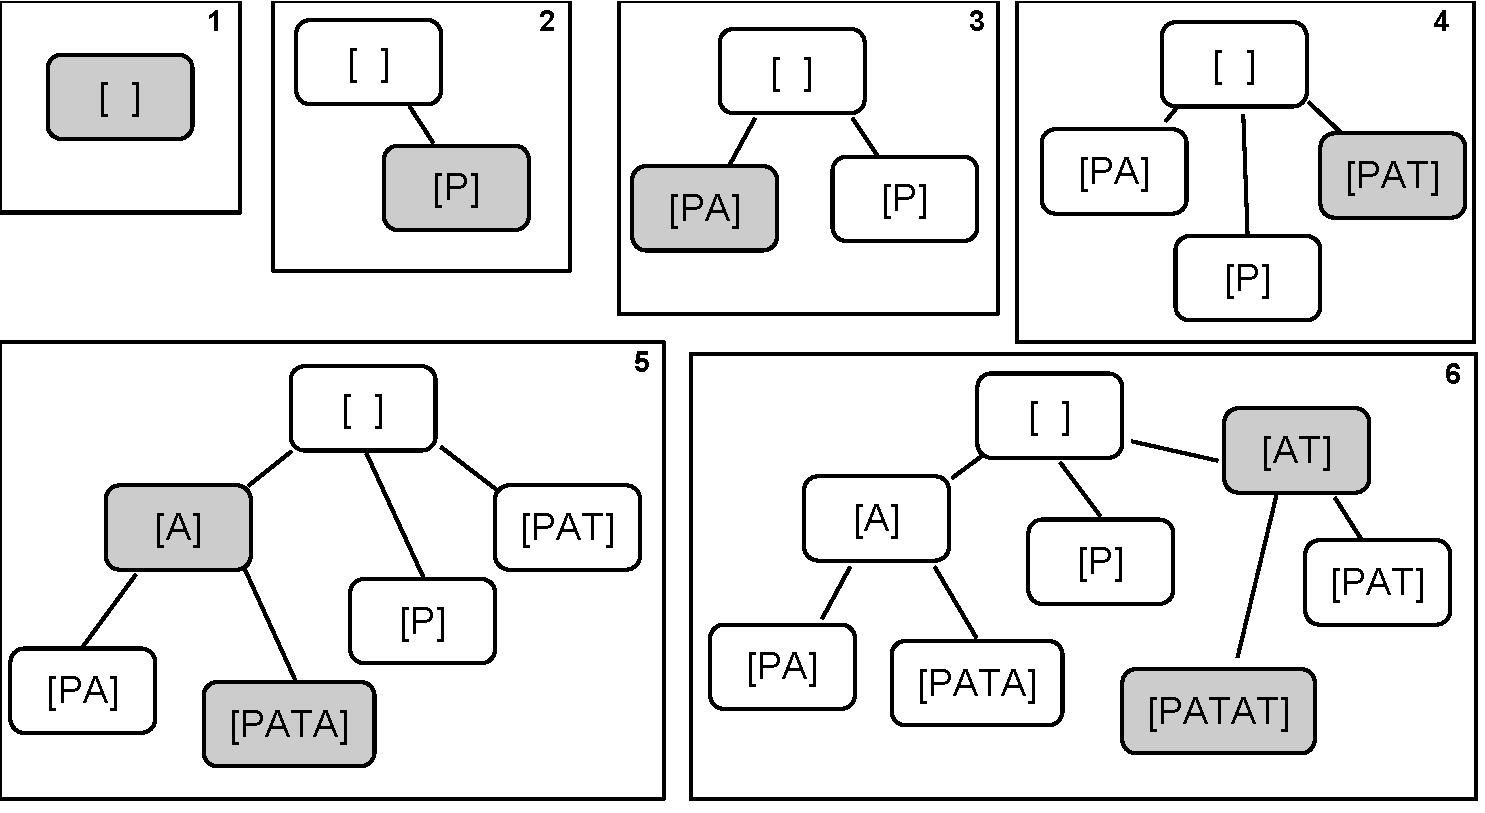
\includegraphics[height = 6cm]{../figs/PATAT.pdf}
		\end{center}
	\end{figure}
\end{frame}


\end{document}
